% !TeX encoding = UTF-8
% !TeX spellcheck = en_US
% !BIB TS-program = biber
% basic packages and document settings
\documentclass[a4paper,12pt]{article}
\usepackage[english]{babel}
\usepackage[utf8]{inputenc}
\usepackage[T1]{fontenc}
\usepackage[a4paper]{geometry}
\geometry{top = 30mm, bottom = 25mm, left = 25mm, right = 25mm}
\usepackage{setspace}
\onehalfspacing
\raggedbottom
\pdfcompresslevel9

% mathmode-related packages
\usepackage{mathtools}
\usepackage{physics}
\usepackage{amsmath}
\usepackage{amsthm}
\usepackage{amsbsy}
\usepackage{mathrsfs}
\usepackage{amssymb}
\usepackage{amstext}
\usepackage{amsfonts}
\usepackage{tikz}
\usepackage{siunitx}
%\usepackage{IEEEtrantools}

% misc
\usepackage{esdiff}
\usepackage{multirow}
\usepackage{blindtext}
\usepackage{todonotes}
\usepackage{abstract}
\usepackage{appendix}
\usepackage[bottom]{footmisc}
\usepackage{listings}
\usepackage{dashrule}

% graphics and floats
\usepackage{graphicx}
\graphicspath{{../Figures/}}
\usepackage{tikz}
\usepackage{float}
\usepackage{wrapfig}
%\usepackage{subfloat}
\usepackage{subcaption}
%\usepackage{caption}
\usepackage[rightcaption]{sidecap}
\usepackage{tabularx}
\usepackage{adjustbox}
%\usepackage{svg}
\usepackage{epstopdf}
\usepackage{grffile}	% handle file names with dots, spaces etc.
%\usepackage{flafter}
\usepackage{rotating}
%\usepackage{floatrow}
%\floatsetup[figure]{capposition=beside,capbesideposition={top,right}}

%\usepackage{epstopdf}
%\epstopdfDeclareGraphicsRule{.pdf}{png}{.png}{convert #1 \OutputFile}
%\AppendGraphicsExtensions{.pdf}

% packages requiring setup arguments

\usepackage{xcolor}
%\definecolor{rwth-dark}{HTML}{176daf}
\definecolor{rwth-dark}{RGB}{0,84,159}
%\definecolor{rwth-light}{HTML}{8abae3}
\definecolor{rwth-light}{RGB}{142,186,229}

%/**
%* Generated by Gpick 0.2.5
%* RWTH Dark: #176daf, rgb(23, 109, 175), hsl(32, 43%, 69%)
%* RWTH Light: #8abae3, rgb(138, 186, 227), hsl(195, 73%, 89%)
%*/

\usepackage{hyperref}
\hypersetup{hidelinks=true,colorlinks=true,allcolors=rwth-dark}
\usepackage[nameinlink,capitalise]{cleveref}
%\usepackage[hyphens]{url}
%\urlstyle{sf}
%\usepackage{breakurl}


% header & footer settings
\usepackage{fancyhdr}
\pagestyle{fancy}
%\renewcommand{\chaptermark}[1]{\markboth{#1}{}} % with this we ensure that the chapter and section headings are in lowercase.
\renewcommand{\sectionmark}[1]{\markright{\thesection\ #1}}
\fancyhf{} % delete current header and footer

%\fancyhead[LE,RO]{\large\thepage}
\fancyhead[L]{\large\rightmark}
\fancyhead[R]{\large\thepage}

\renewcommand{\headrulewidth}{0.3pt}
\renewcommand{\footrulewidth}{0pt}
%\addtolength{\headheight}{0.5pt} % space for the rule

\fancyfoot[C]{\thepage}

\fancypagestyle{plain}
{
	\fancyhead{} % get rid of headers on plain pages
	\renewcommand{\headrulewidth}{0pt} % and the line
}

% ========== command definitions =================================
\newcommand{\Thickline}{\rule{\linewidth}{0.4mm}}
\newcommand{\Thinline}{\rule{\linewidth}{0.1mm}}

\newcommand{\id}{\, \mathrm{d}}

\definecolor{codegray}{gray}{0.9}
\newcommand{\code}[1]{\colorbox{codegray}{\texttt{#1}}}

\newcommand{\skippage}{\clearpage{\thispagestyle{empty}\cleardoublepage}}

\def\@esphack{%
	\relax
	\ifhmode
	\spacefactor\@savsf
	\ifdim\@savsk>\z@
	\ignorespaces
	\fi
	\fi}

\title{\LARGE title}
\date{}


\begin{document}
	
\begin{titlepage}
	\thispagestyle{empty}
	\newgeometry{top=20mm, left=20mm, right=20mm, bottom=20mm}
	
%	\begin{minipage}{0.35\textwidth}
%		\begin{flushleft}
%
%
%		\end{flushleft}
%	\end{minipage}
%	\hfill
%	\begin{minipage}{0.65\textwidth}
%		\begin{flushright}
%
%		\end{flushright}
%	\end{minipage}
	
%	\vspace*{\fill}
	\hspace{0pt}
	\vspace{2cm}
	\begin{center}
%		\Thickline
%		\vskip -0.5cm
%		\Thinline
		\hdashrule{\linewidth}{1pt}{}
		\vskip -0.5cm
		\hdashrule{\linewidth}{0.5pt}{}
		
		\vspace{0.5cm}
		\Huge{ \textbf{ F3 \\}}
		\LARGE{ \textbf{Rastertunnelmikroskopie} } 
		
		\hdashrule{\linewidth}{0.5pt}{}
		\vskip -0.95cm
		\hdashrule{\linewidth}{1pt}{}
%		\Thinline
%		\vskip -0.9cm
%		\Thickline 
		
		\vspace{3cm}
		\Large{\textbf{ Gruppe 14 \\}}
		\Large{Heithem Assili, 368441 \\ Alexandre Drouet, 355095 \\ Olexiy Fedorets, 356615 \\}
		\vspace{1cm}
		\Large{\textsl{ Versuchstag: 12.03.2019 \\ Protokollabgabe: 27.03.2019}}

		

		
	\end{center}
	\vfill
%	\vspace*{\fill}
	
\end{titlepage}
	
	
	
\skippage
\pagenumbering{roman}
\thispagestyle{plain}

\tableofcontents
%	\newpage
\newpage
\listoffigures

%\begingroup
%\let\cleardoublepage\relax
%\let\clearpage\relax
\listoftables
%\endgroup
%\listoftables

\skippage

\pagenumbering{arabic}
\setcounter{page}{1}
\restoregeometry
\thispagestyle{fancy}


\section{Einleitung}

In diesem Versuch beschäftigen wir uns mit einem Rastertunnelmikroskop (RTM). Erstmal ist das Ziel sich mit der Funktionsweise und den Einstellmöglichkeiten des Mikroskops vertraut zu machen um später die atomare Auflösung zu demonstrieren und den Rasterbereich zu kalibrieren.

\subsection{Theorie und Prinzip des RTM}

Das Rastertunnelmikroskop basiert wie der Name schon andeutet auf den Tunneleffekt. Eine Spitze rastert bei angelegter Tunnelspannung einen Bereich einer Probe ab, so dass nur tunnelnde Elektronen zu einem Strom beitragen. Die feine Rasterbewegung wird realisiert durch drei Piezokristalle, einen für jede Raumrichtung. Diese erlauben präzise Bewegung im Subnanometerbereich.

Ein RTM hat zwei wesentliche Betriebsmodi. Einerseits den Konstantstrommodus, in dem der Strom möglichst konstant gehalten wird durch Regelung der Höhe, also Bewegung in z-Richtung. In diesem Fall ist die Topographie im z-Bild sichtbar. Andererseits gibt es den Konstanthöhenmodus bei dem die Spitze bei konstanter Höhe über die Probe fährt und die Topographie im Strombild sichtbar wird. Es kann von einem Modus in den anderen gewechselt werden über die Einstellung der Höhenregelung (über Gain und Rasterzeit). Der Konstanthöhenmodus ist der Grenzfall des Konstantstrommodus bei dem die Höhenregelung sehr langsam ist.

\section{Aufbau}

In diesem Versuch verwenden wir ein RTM der Marke Nanosurf. Die Tunnelspitze haben wir selber aus einem Draht erstellt. Die Spitze wird in eine Mulde gelegt und von einer Feder festgehalten. Die Probe wird auf einem Magnetsockel gelegt der wiederum auf einer Halterung mit Schrittmotor aufliegt.

Zum groben Anfahren wird der Schrittmotor verwendet, bevor für die vorsichtige Annäherung und das Rastern die Piezokristalle verwendet werden. 

\begin{figure}[H]
\centering
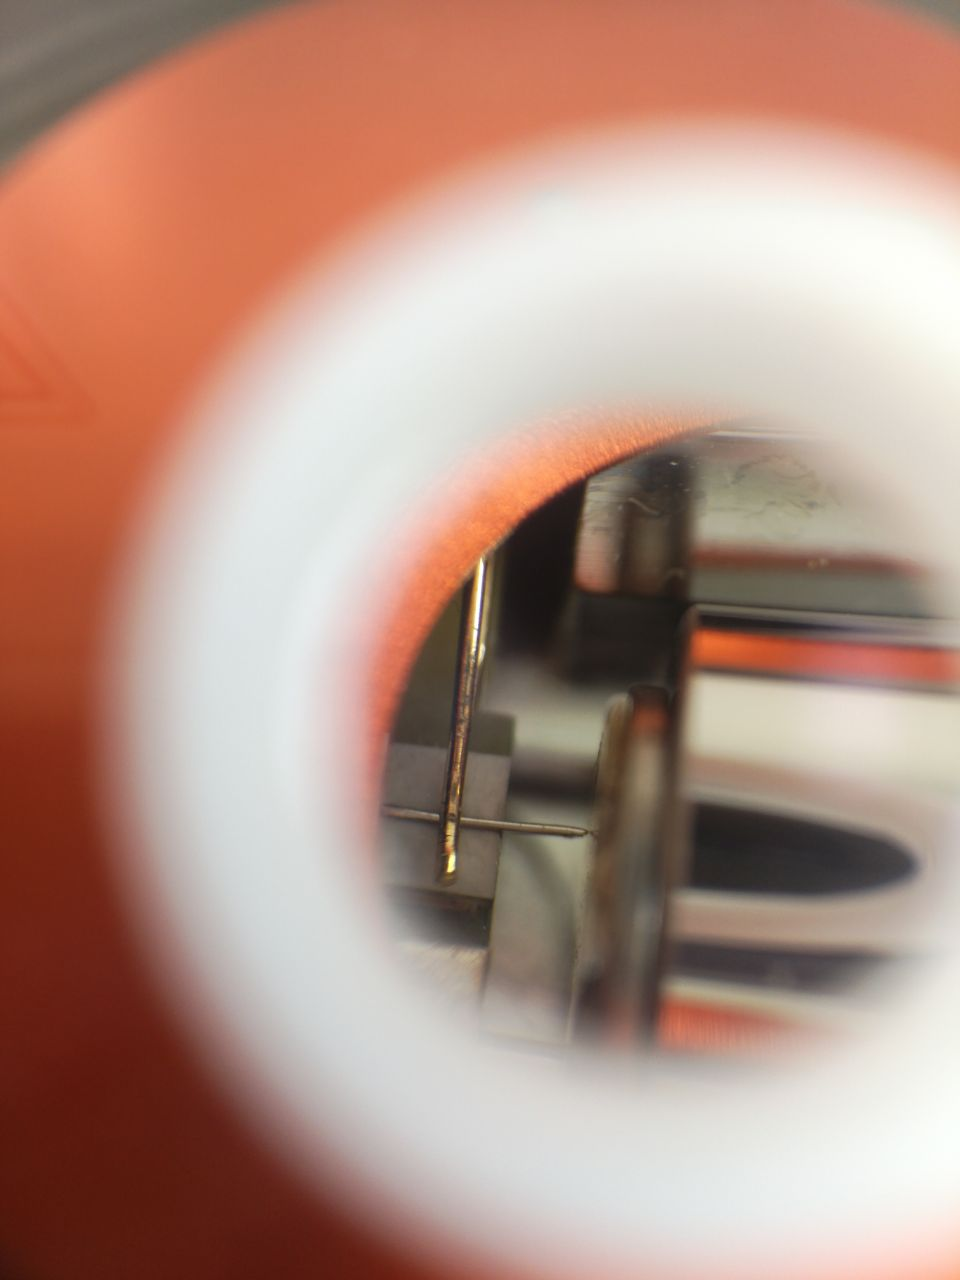
\includegraphics[width=\textwidth]{../RTM.jpg}
\caption{Tunnelspitze mit Probe gesehen durch eine Linse.}
\label{RTM}
\end{figure}

\section{Durchführung und Auswertung}
Für die Auswertung der RTM-Bilder nutzen wir Gwyddion 2.50. Mithilfe von Gwyddion extrahierte Daten haben wir wiederrum mit Python 3.6 ausgewertet. 

\subsection{Gold}

\begin{figure}[H]
\centering
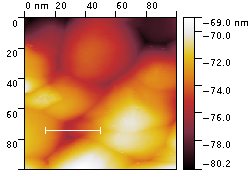
\includegraphics[width=\textwidth]{../Gwyddion/Gold/GAIN_opt_Z_forward.pdf}
\caption{Z-Bild der untersuchten Goldprobe bei Gain 1900 und Rasterzeit \SI{0.1}{s}.}
\label{GAIN_opt_Z}
\end{figure}

Als erstes wollen wir eine Goldprobe untersuchen und uns anhand dieser mit der Funktionsweise des RTM vertraut machen. Dazu suchen wir uns eine charakteristische Stelle auf der Probe (siehe Abbildung \ref{GAIN_opt_Z}) und nehmen Bilder mit unterschiedlichen Einstellungen auf. Erst variieren wir den I-Gain und nehmen vier unterschiedliche Bilder auf. Danach halten wir die beste Einstellung fest, variieren die Rasterzeit und nehmen wieder unterschiedliche Bilder auf.

Bei der Betrachtung der Strombilder für unterschiedliche I-Gains, fällt auf, dass für geringere Gains, also langsamere Regelung, immer mehr von der Topographie sichtbar wird. Für höhere Gains sehen wir immer mehr weiße Punkte durch Übersteuerung und wellenartige Muster.

\begin{figure}[H]
\centering
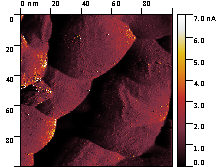
\includegraphics[width=\textwidth]{../Gwyddion/Gold/GAIN_slow_I_forward.pdf}
\caption{Strombild der untersuchten Goldprobe bei Gain 800 und Rasterzeit \SI{0.1}{s}.}
\label{GAIN_slow_I}
\end{figure}

\begin{figure}[H]
\centering
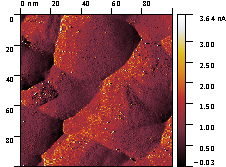
\includegraphics[width=\textwidth]{../Gwyddion/Gold/GAIN_opt_I_forward.pdf}
\caption{Strombild der untersuchten Goldprobe bei Gain 1900 und Rasterzeit \SI{0.1}{s}.}
\label{GAIN_opt_I}
\end{figure}

\begin{figure}[H]
\centering
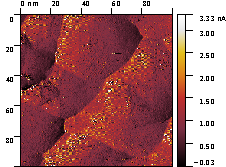
\includegraphics[width=\textwidth]{../Gwyddion/Gold/GAIN_extra_I_forward.pdf}
\caption{Stromild der untersuchten Goldprobe bei Gain 2500 und Rasterzeit \SI{0.1}{s}.}
\label{GAIN_extra_I}
\end{figure}

\begin{figure}[H]
\centering
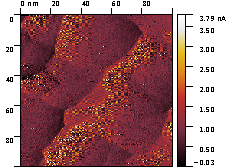
\includegraphics[width=\textwidth]{../Gwyddion/Gold/GAIN_fast_I_forward.pdf}
\caption{Strombild der untersuchten Goldprobe bei Gain 3000 und Rasterzeit \SI{0.1}{s}.}
\label{GAIN_fast_I}
\end{figure}

Als optimalen Gain haben wir 1900 gewählt, da es einen guten Kompromiss zwischen beiden Extremen darstellt. Um das quantitativ zu begründen haben wir erstmal die Profile der z-Bilder für die Gains 1900 und 800 jeweils in Vor- und Rückwärtsrichtung an der selben Stelle extrahiert. Man erkennt klar, dass die Veschiebung zwischen beide Richtungen beim kleineren Gain deutlich größer ist. Nach Bestimmung der Minima und Berechnung der Differenz (auf der x-Achse) ergibt sich für einen Gain von 1900 bzw. 800 eine Verschiebung um \SI{5,08}{nm} bzw. \SI{8,98}{nm}.

\begin{figure}[H]
\centering
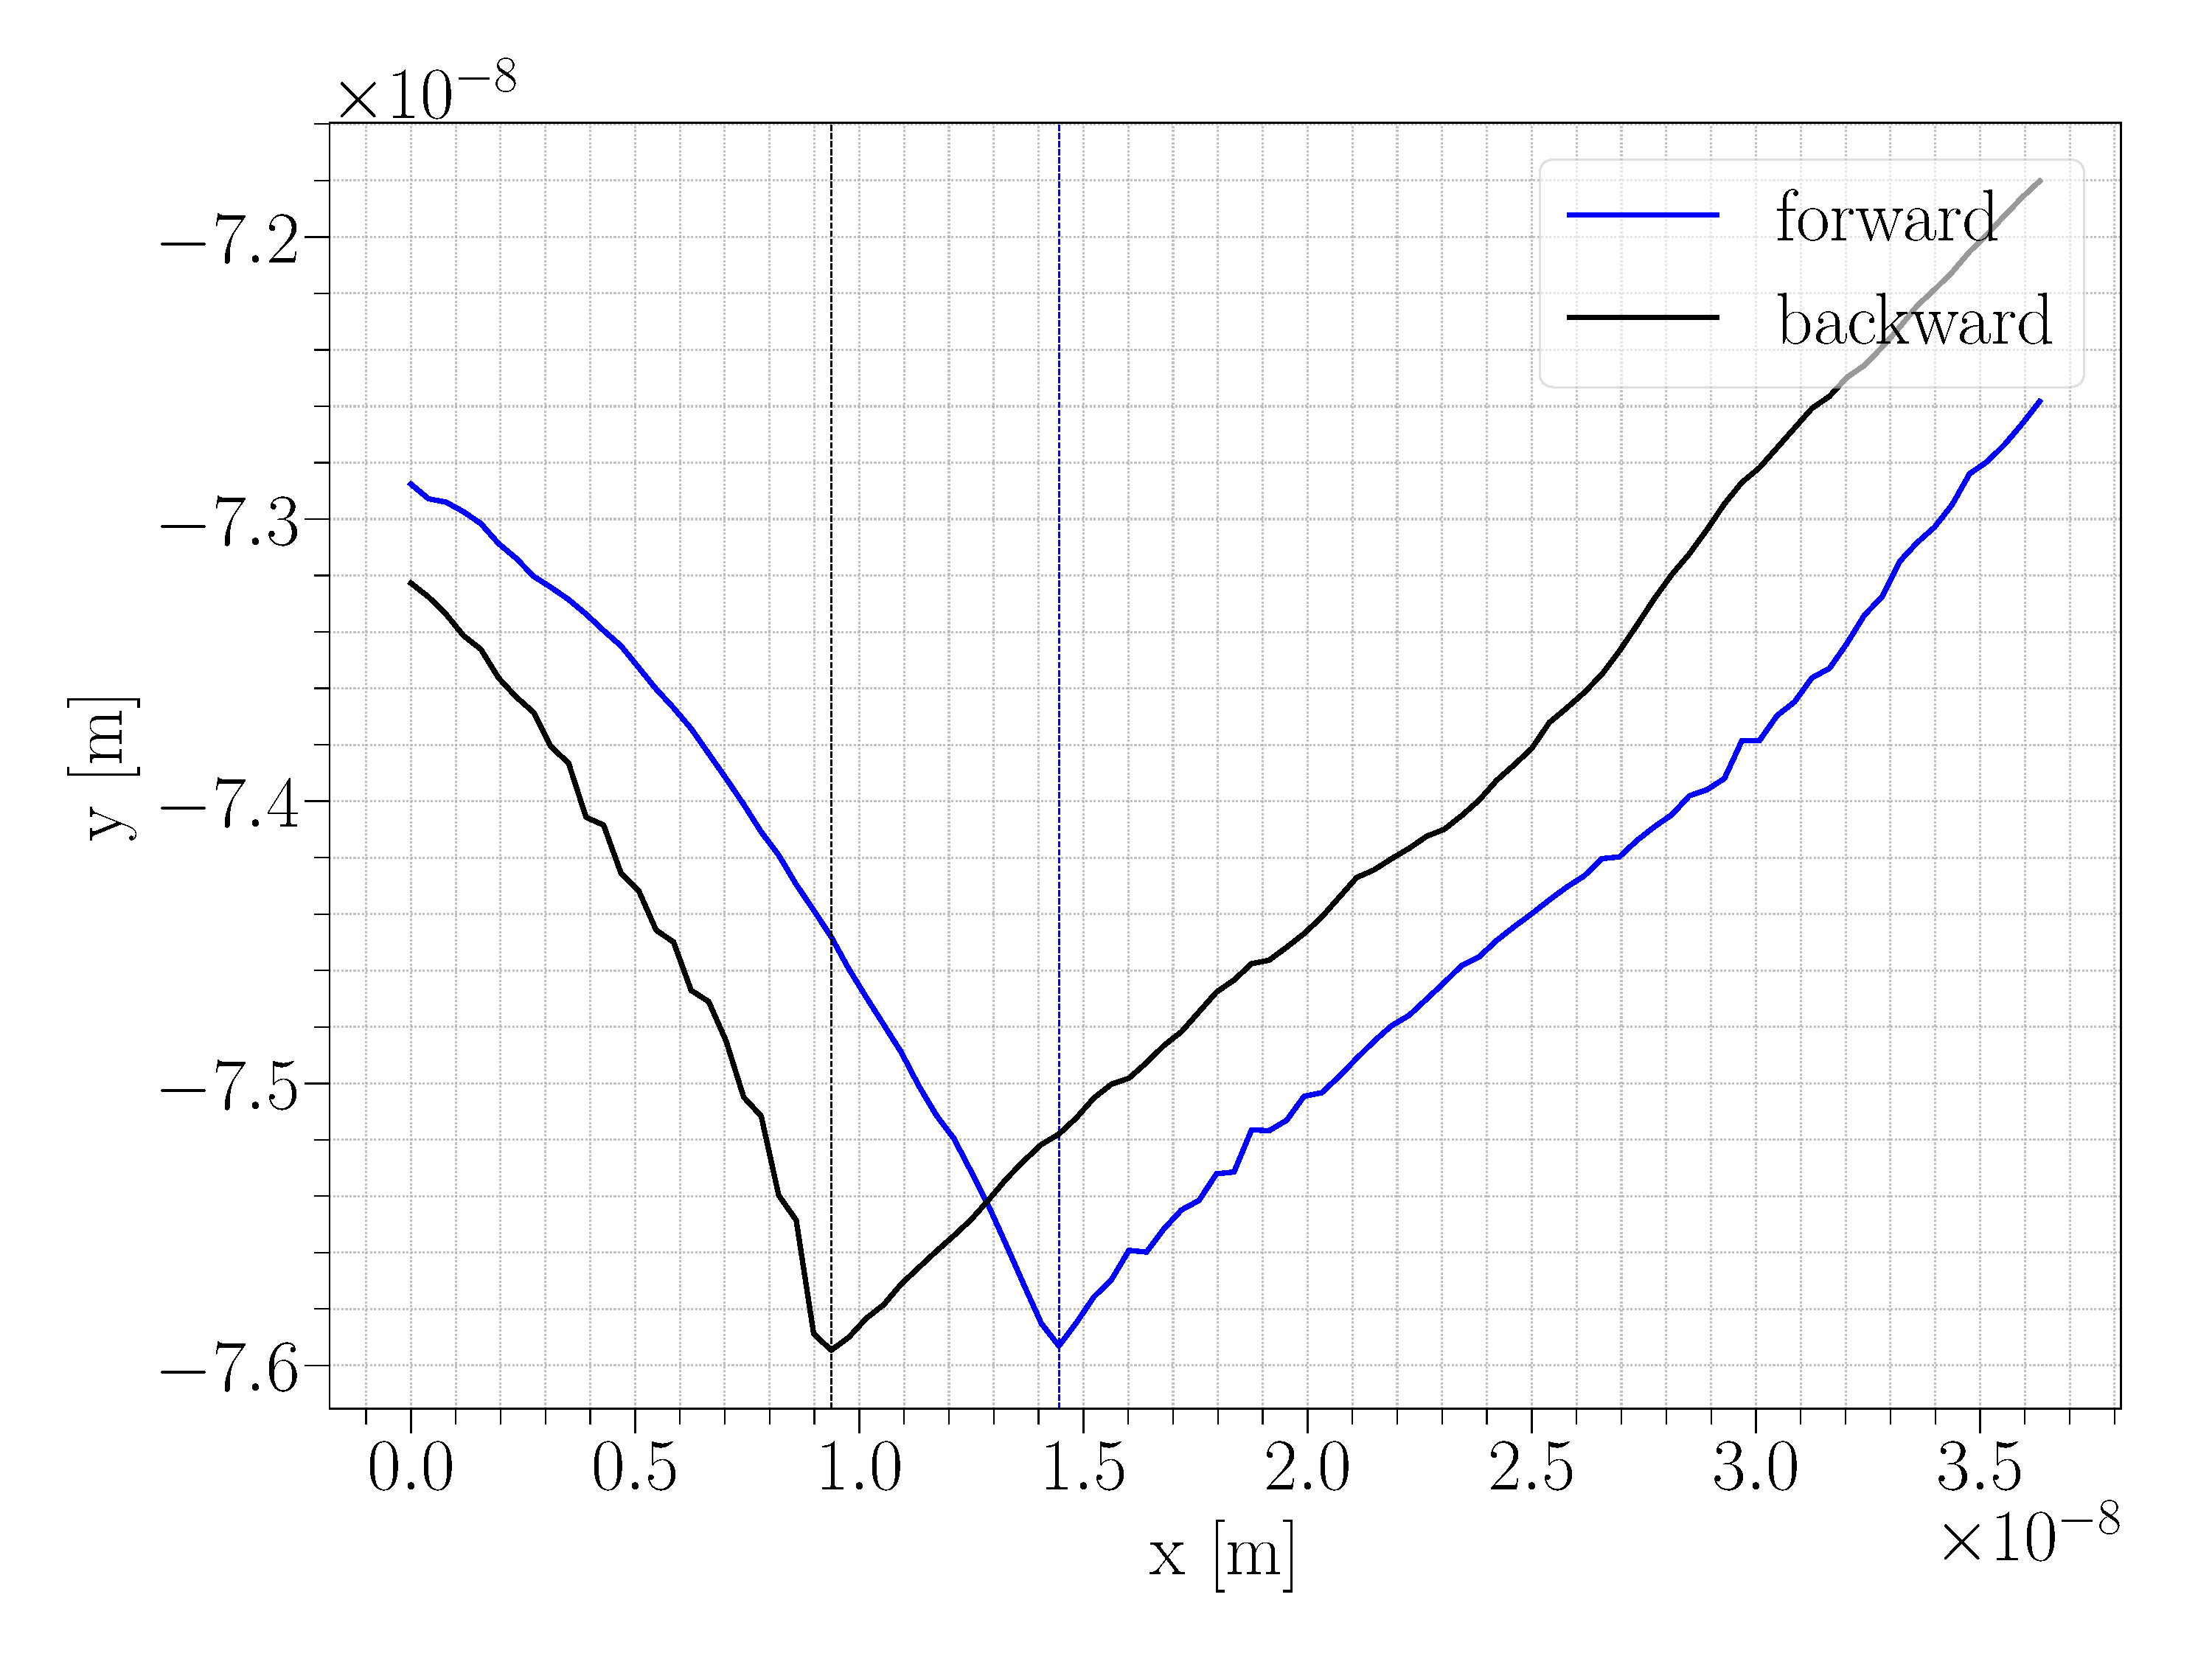
\includegraphics[width=\textwidth]{../Figures/GAIN_opt_profile.pdf}
\caption{Extrahierte Profile in Vor- und Rückwärtsrichtung für einen Gain von 1900.}
\label{GAIN_opt_profile}
\end{figure}

\begin{figure}[H]
\centering
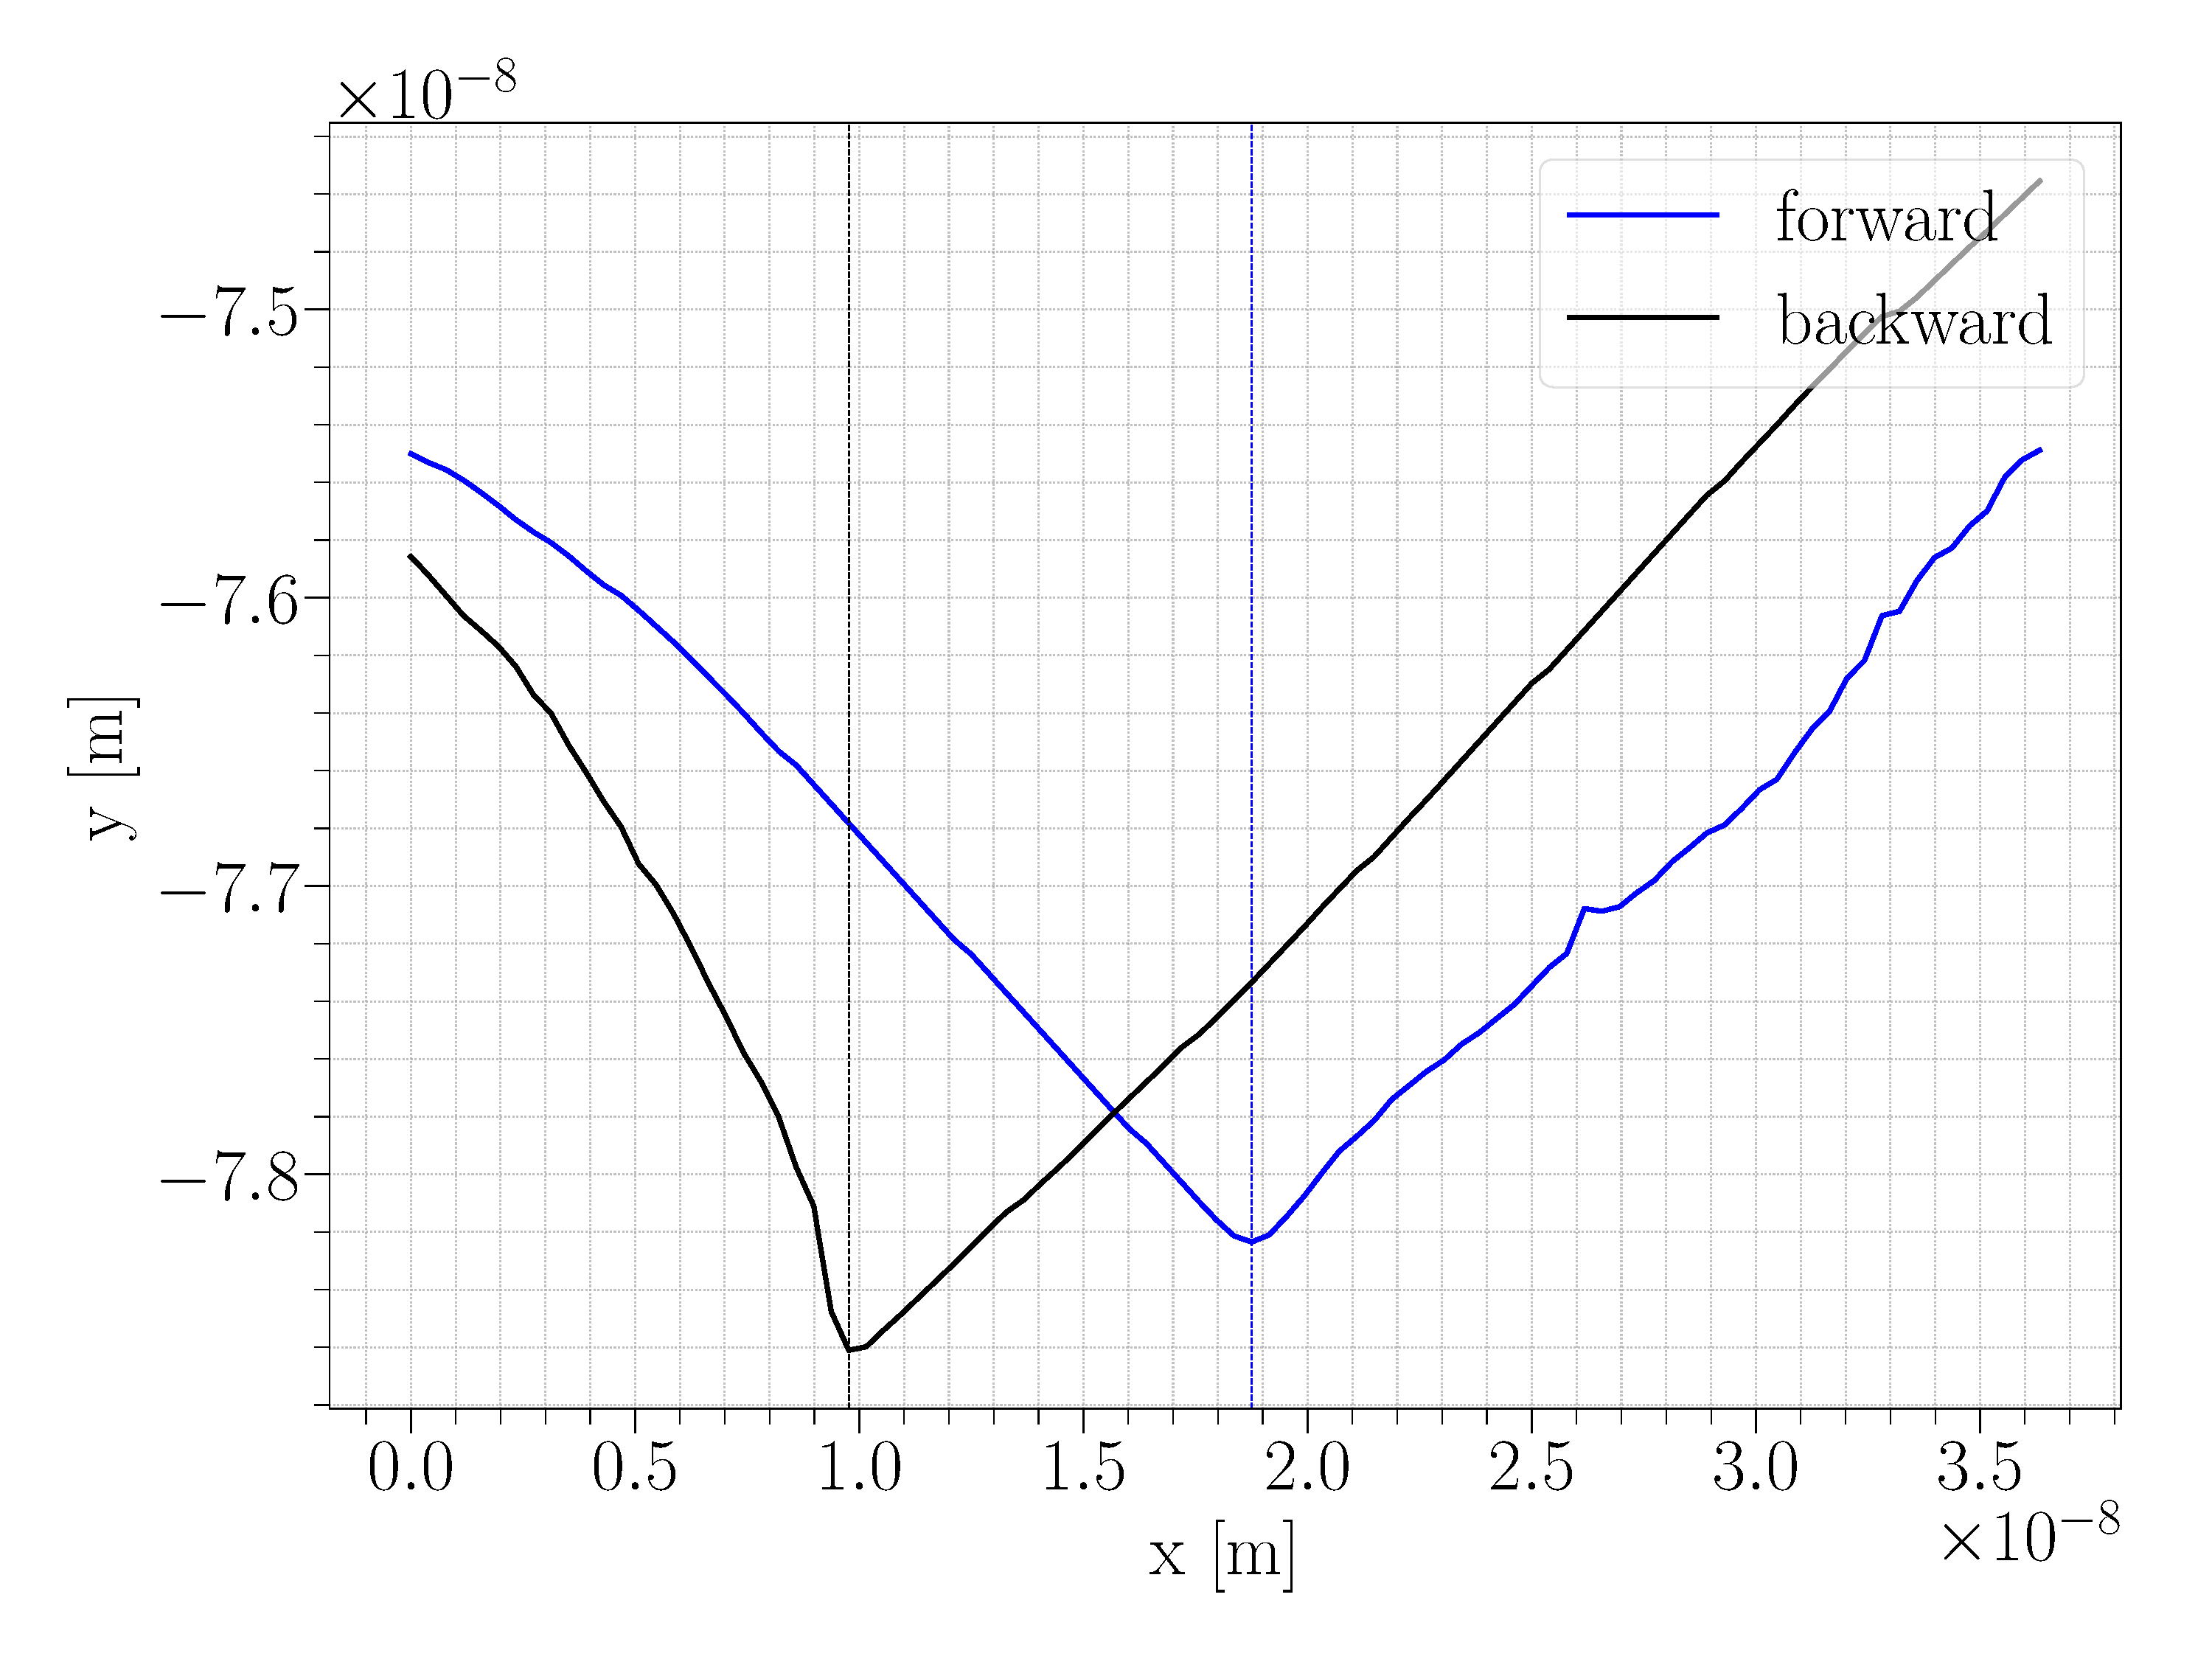
\includegraphics[width=\textwidth]{../Figures/GAIN_slow_profile.pdf}
\caption{Extrahierte Profile in Vor- und Rückwärtsrichtung für einen Gain von 800.}
\label{GAIN_slow_profile}
\end{figure}

Um den Gain nach oben abzugrenzen, schauen wir uns die Profile identischer Stellen im Strombild für Gain 1900 und 2500 an. Nun bestimmen wir im selben Bereich (10 bis \SI{20}{nm}) jeweils die Peak-to-Peak-Amplitude, also die Differenz zwischen globalem Maximum und globalem Minimum in diesem Bereich (siehe Abbildung \ref{GAIN_I_forward_profiles}). Diese Zahl nehmen wir hier als Maß für die Oszillation bzw. Übersteuerung. Wir finden für einen Gain von 1900 bzw. 2500 eine Amplitude von \SI{5,05e-10}{A} bzw. \SI{8,34e-10}{A}. Damit oszilliert das Strombild beim Gain von 1900 merklich weniger. 

\begin{figure}[H]
\centering
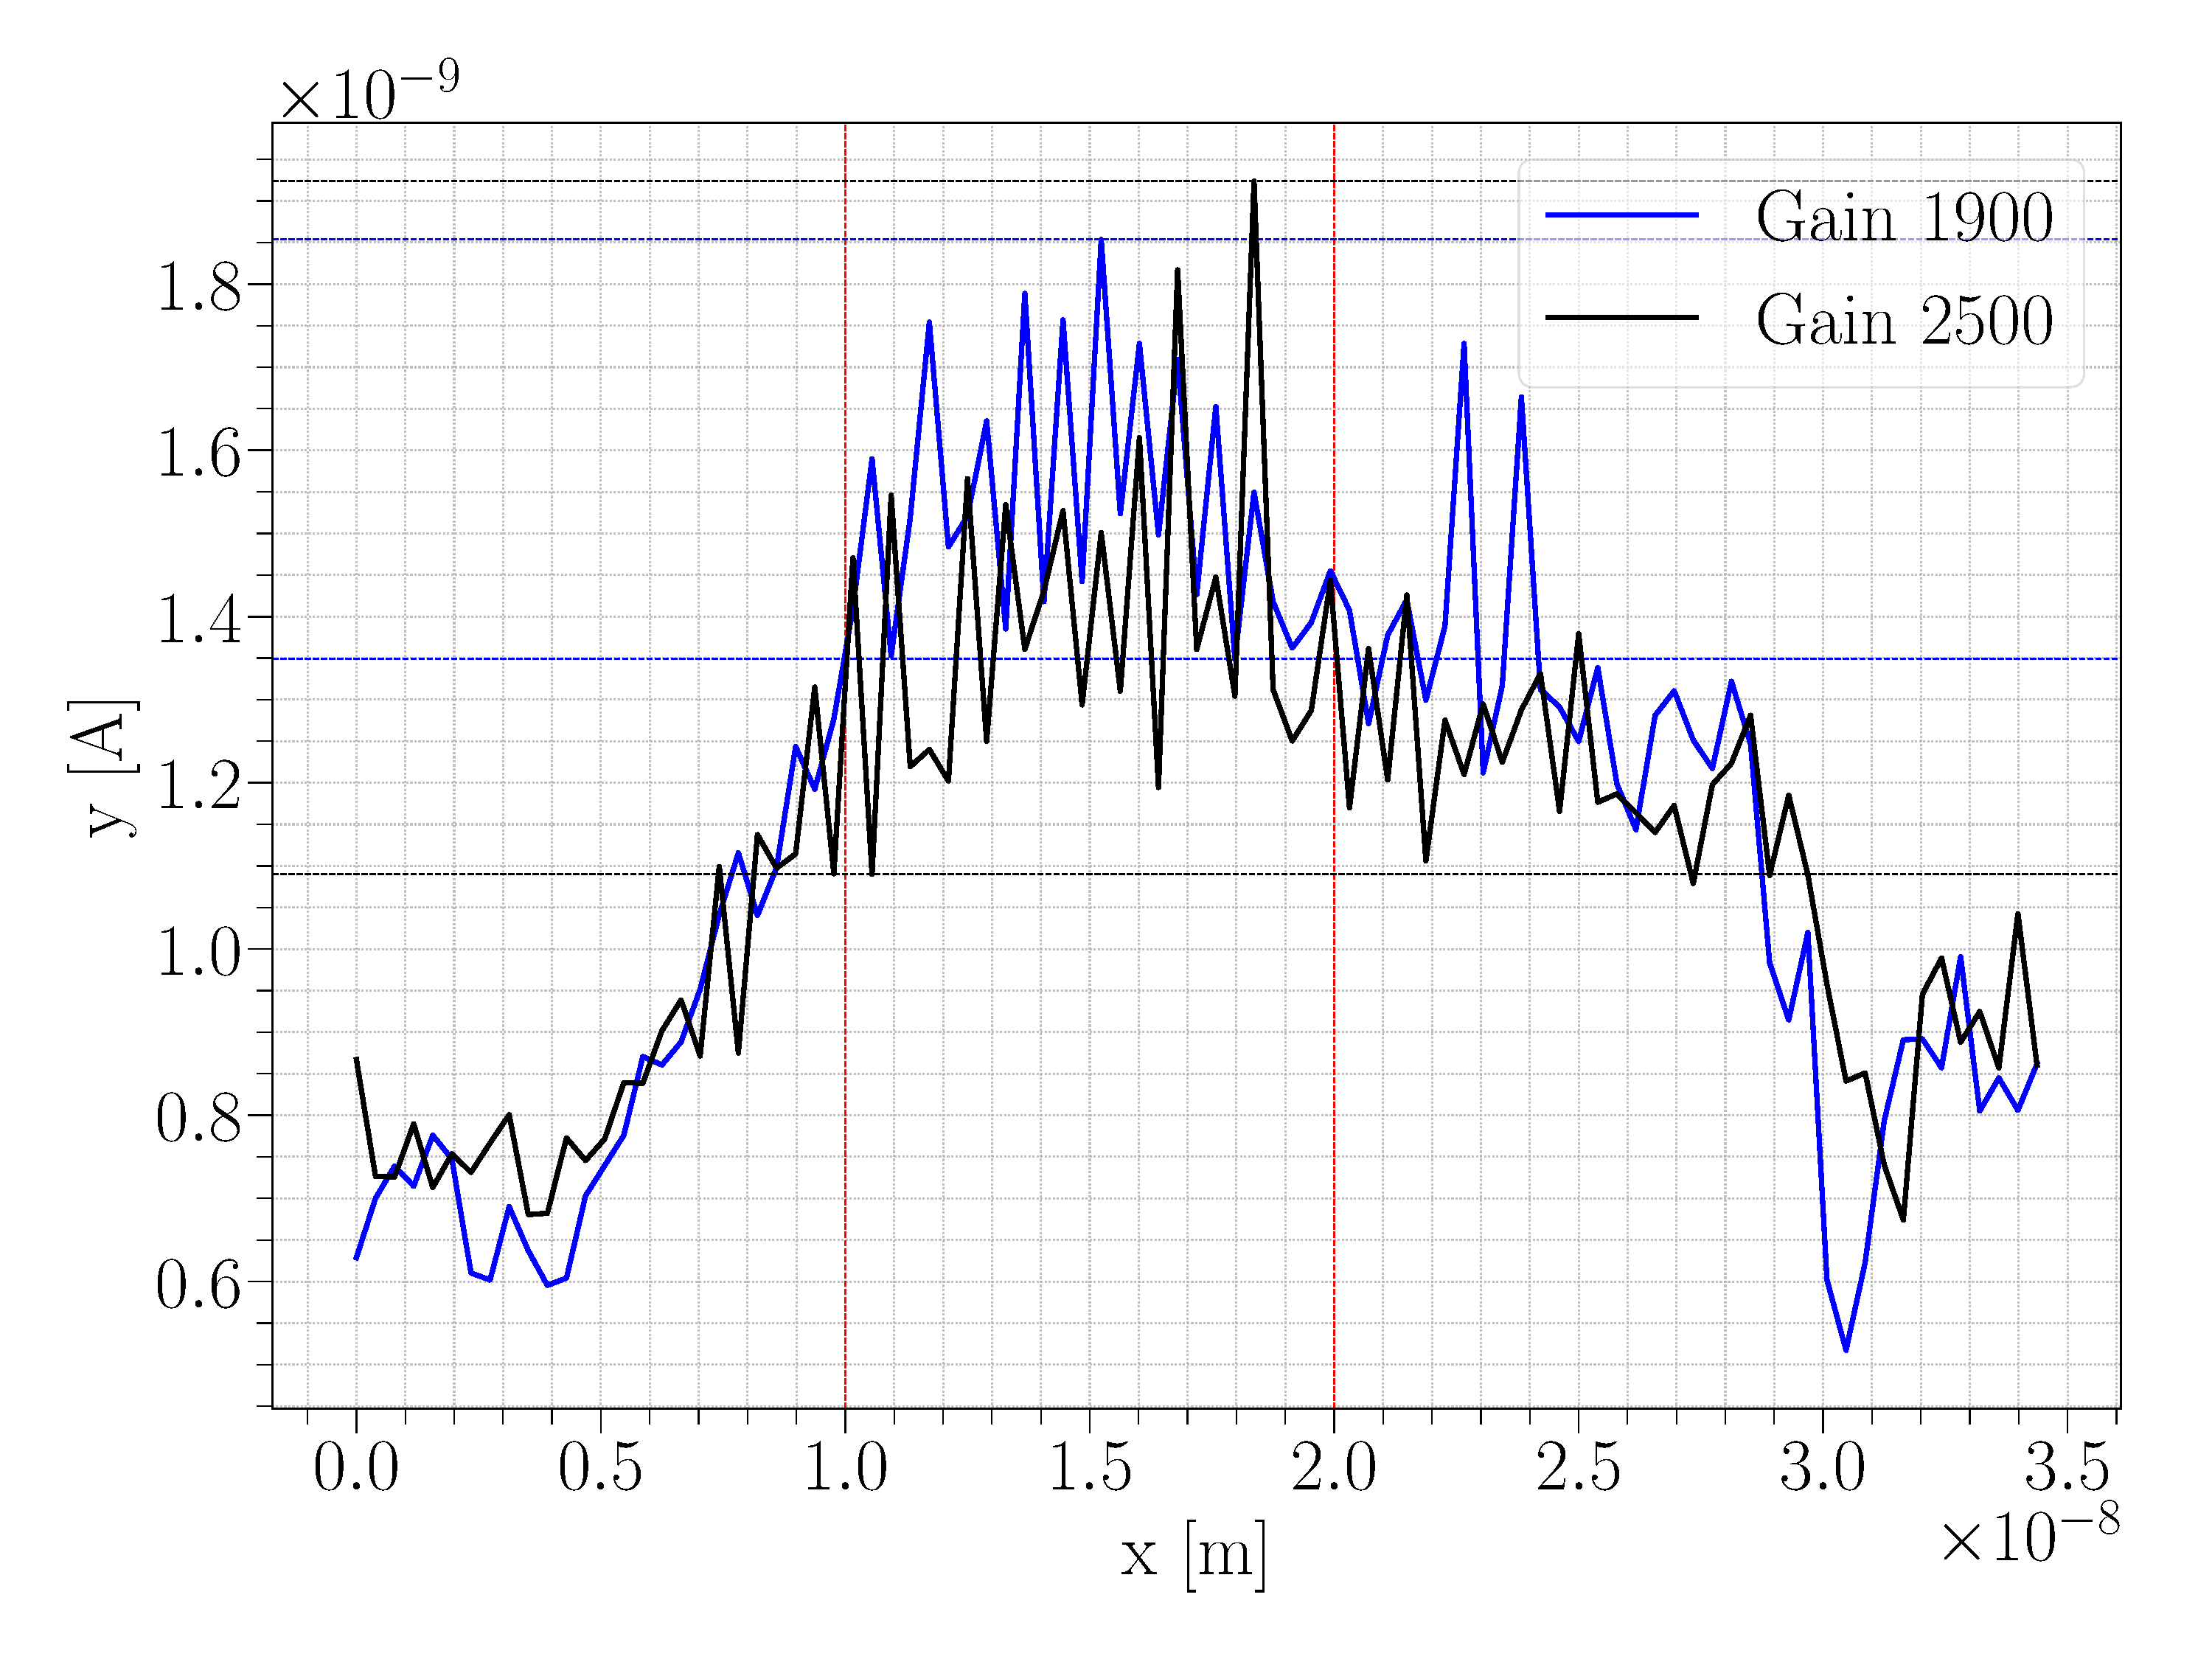
\includegraphics[width=\textwidth]{../Figures/GAIN_I_forward_profiles.pdf}
\caption{Aus dem Strombild extrahierte Profile. Horizontale Linien markieten die gefundenen Extrema, vertikale Linien markieren die Ränder des betrachteten Bereichs.}
\label{GAIN_I_forward_profiles}
\end{figure}

Bei der Variierung der Rasterzeit lassen sich im Strombild ganz ähnliche Effekte wie beim Gain beobachten, wobei eine kleinere Rasterzeit der Regelung weniger Zeit zum reagieren gibt und somit einem kleineren Gain entspricht. Das Umgekehrte gilt nicht umbedingt für größere Rasterzeiten, aber dafür beobachten wir ein zunehmends verauschteres Bild.

\begin{figure}[H]
\centering
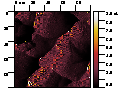
\includegraphics[width=\textwidth]{../Gwyddion/Gold/TIME_005_I_forward.pdf}
\caption{Strombild der untersuchten Goldprobe bei Gain 1900 und Rasterzeit \SI{0.05}{s}.}
\label{TIME_005_I}
\end{figure}

\begin{figure}[H]
\centering
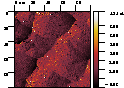
\includegraphics[width=\textwidth]{../Gwyddion/Gold/TIME_01_I_forward.pdf}
\caption{Strombild der untersuchten Goldprobe bei Gain 1900 und Rasterzeit \SI{0.1}{s}.}
\label{TIME_01_I}
\end{figure}

\begin{figure}[H]
\centering
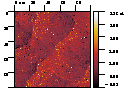
\includegraphics[width=\textwidth]{../Gwyddion/Gold/TIME_02_I_forward.pdf}
\caption{Strombild der untersuchten Goldprobe bei Gain 1900 und Rasterzeit \SI{0.2}{s}.}
\label{TIME_02_I}
\end{figure}

\begin{figure}[H]
\centering
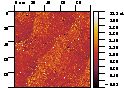
\includegraphics[width=\textwidth]{../Gwyddion/Gold/TIME_04_I_forward.pdf}
\caption{Strombild der untersuchten Goldprobe bei Gain 1900 und Rasterzeit \SI{0.4}{s}.}
\label{TIME_04_I}
\end{figure}

Als optimale Rasterzeit haben wir \SI{0,1}{s} gewählt. Bei der quantitativen Begündung verfahren wir analog zur Variierung des Gains. Vergleichen wir die entsprechenden Profile der z-Bilder, finden wir für \SI{0,1}{s} bzw. \SI{0,05}{s} eine Verschiebung zwischen Vor- und Rückwärtsrichtung von \SI{6,25}{nm} bzw. \SI{7,81}{nm}.

\begin{figure}[H]
\centering
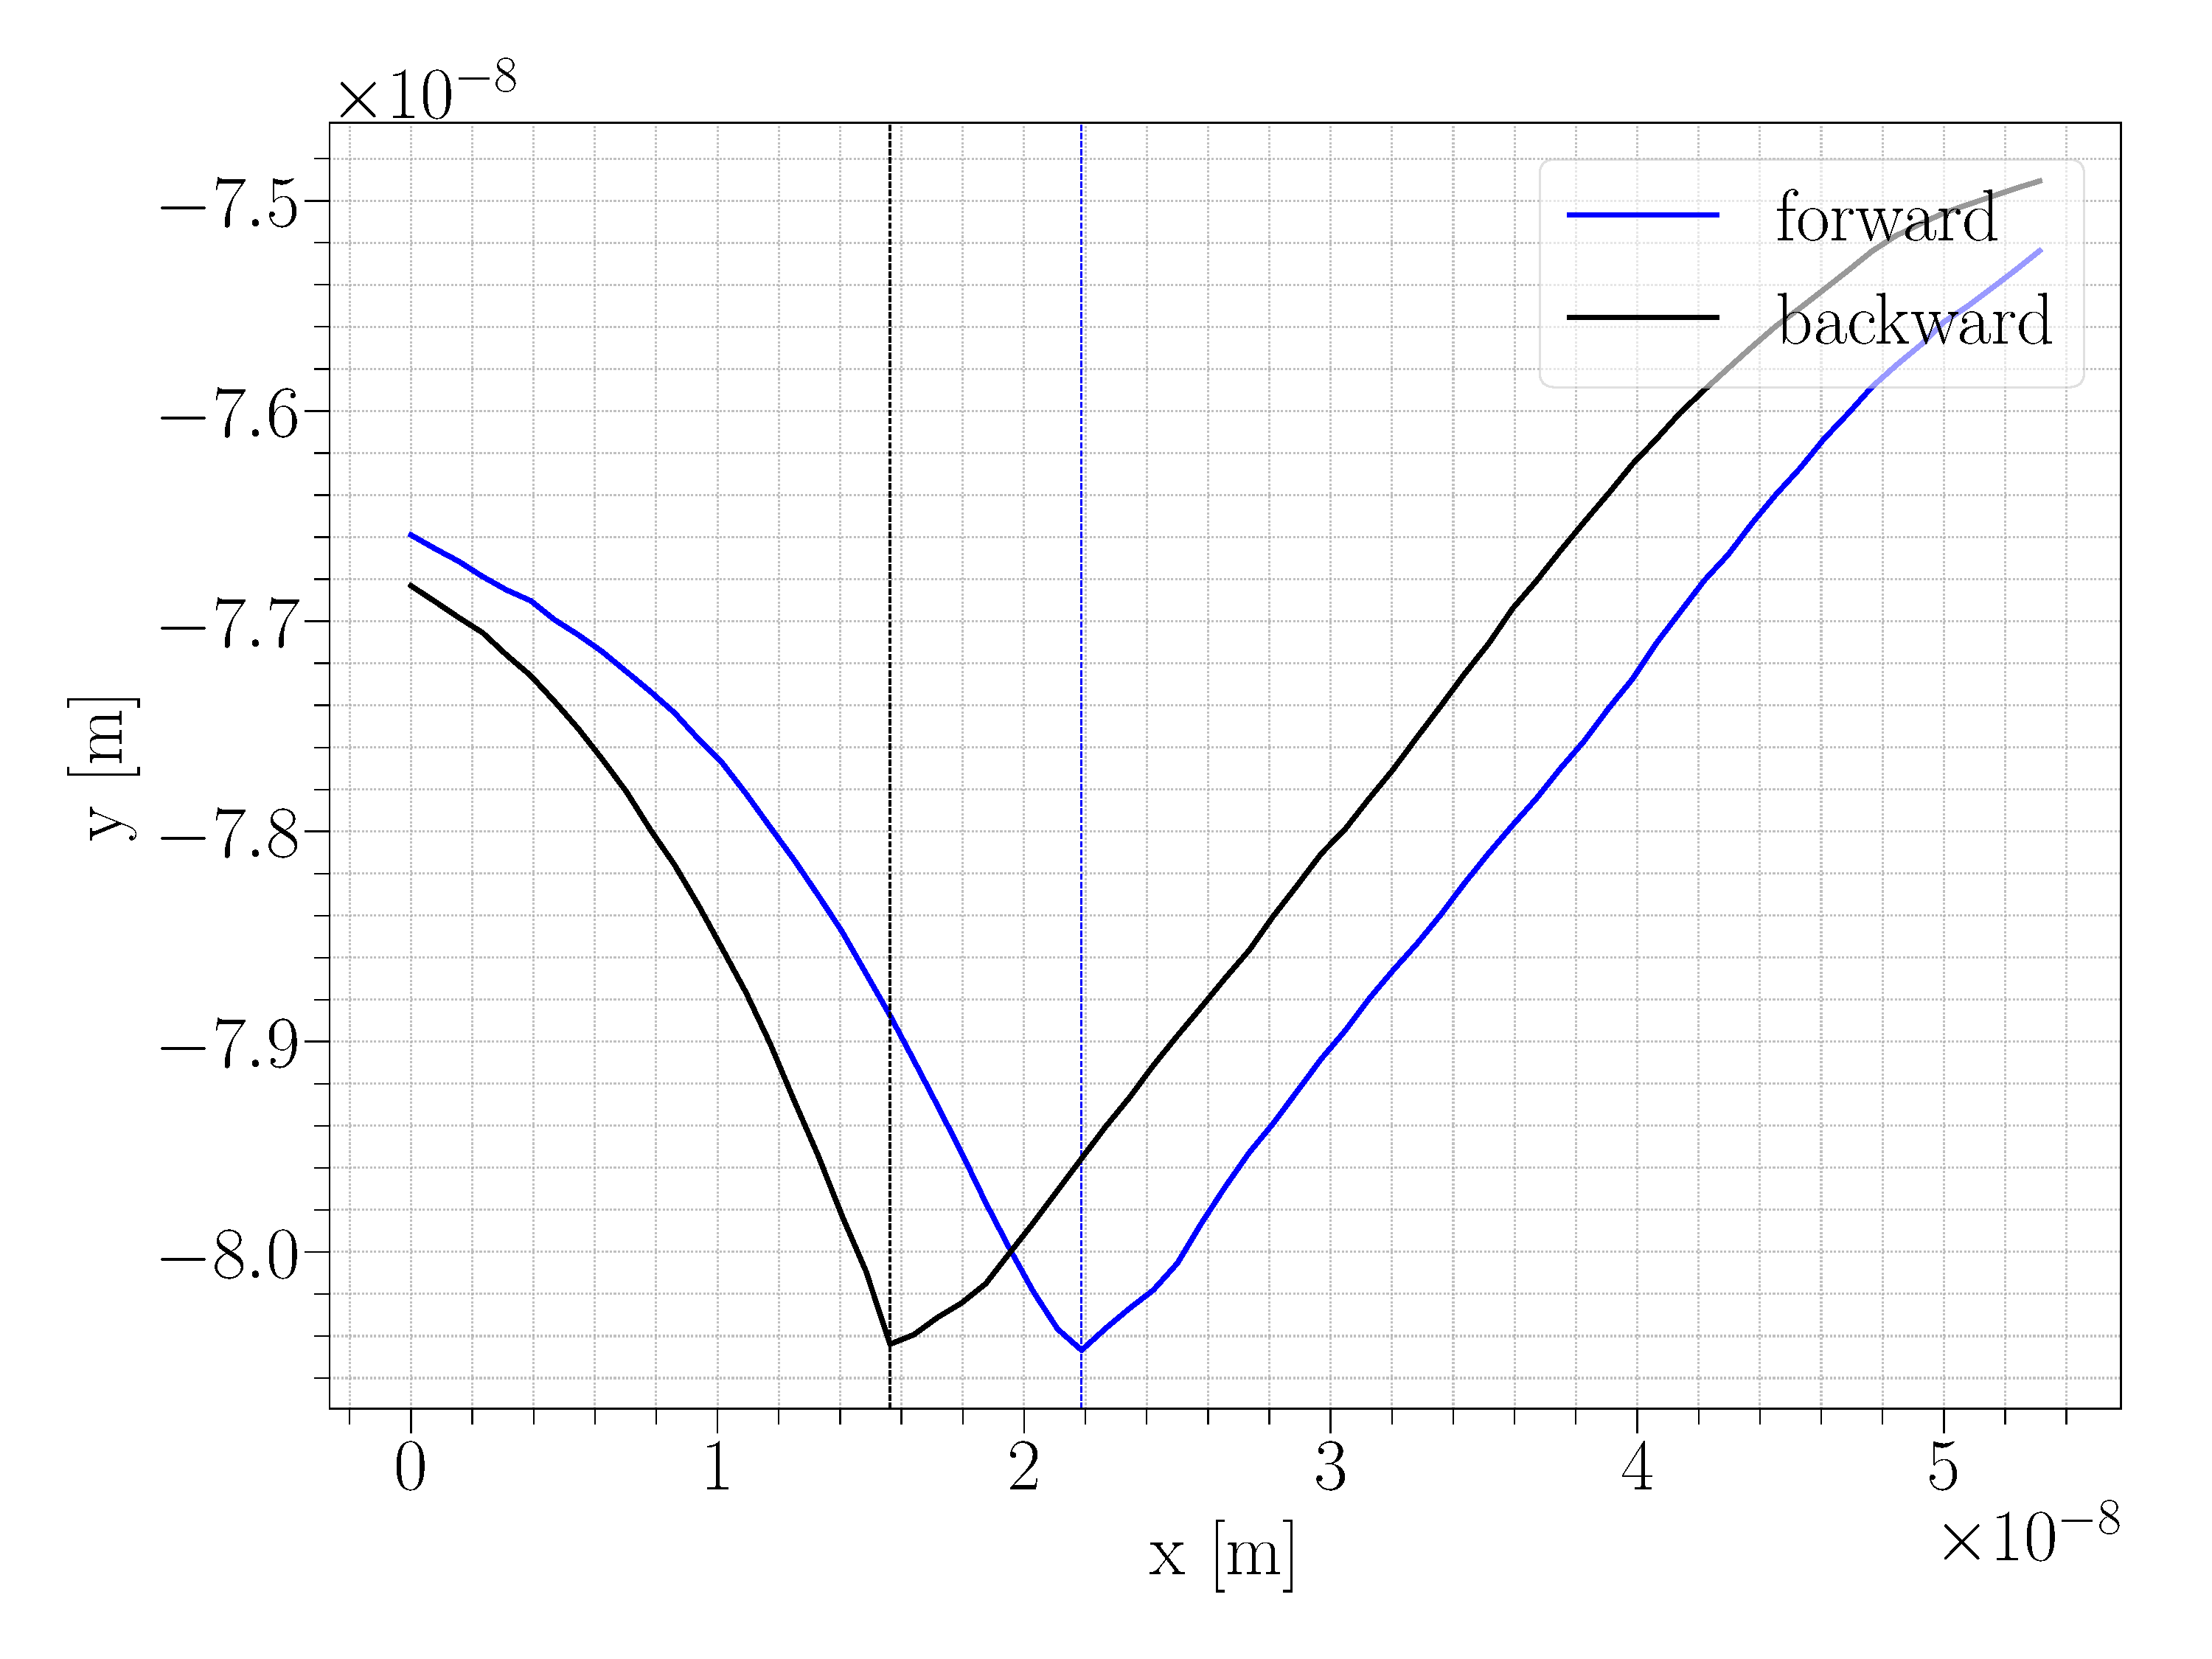
\includegraphics[width=\textwidth]{../Figures/TIME_01_profile.pdf}
\caption{Extrahierte Profile in Vor- und Rückwärtsrichtung für eine Rasterzeit von \SI{0.1}{s}.}
\label{TIME_01_profile}
\end{figure}

\begin{figure}[H]
\centering
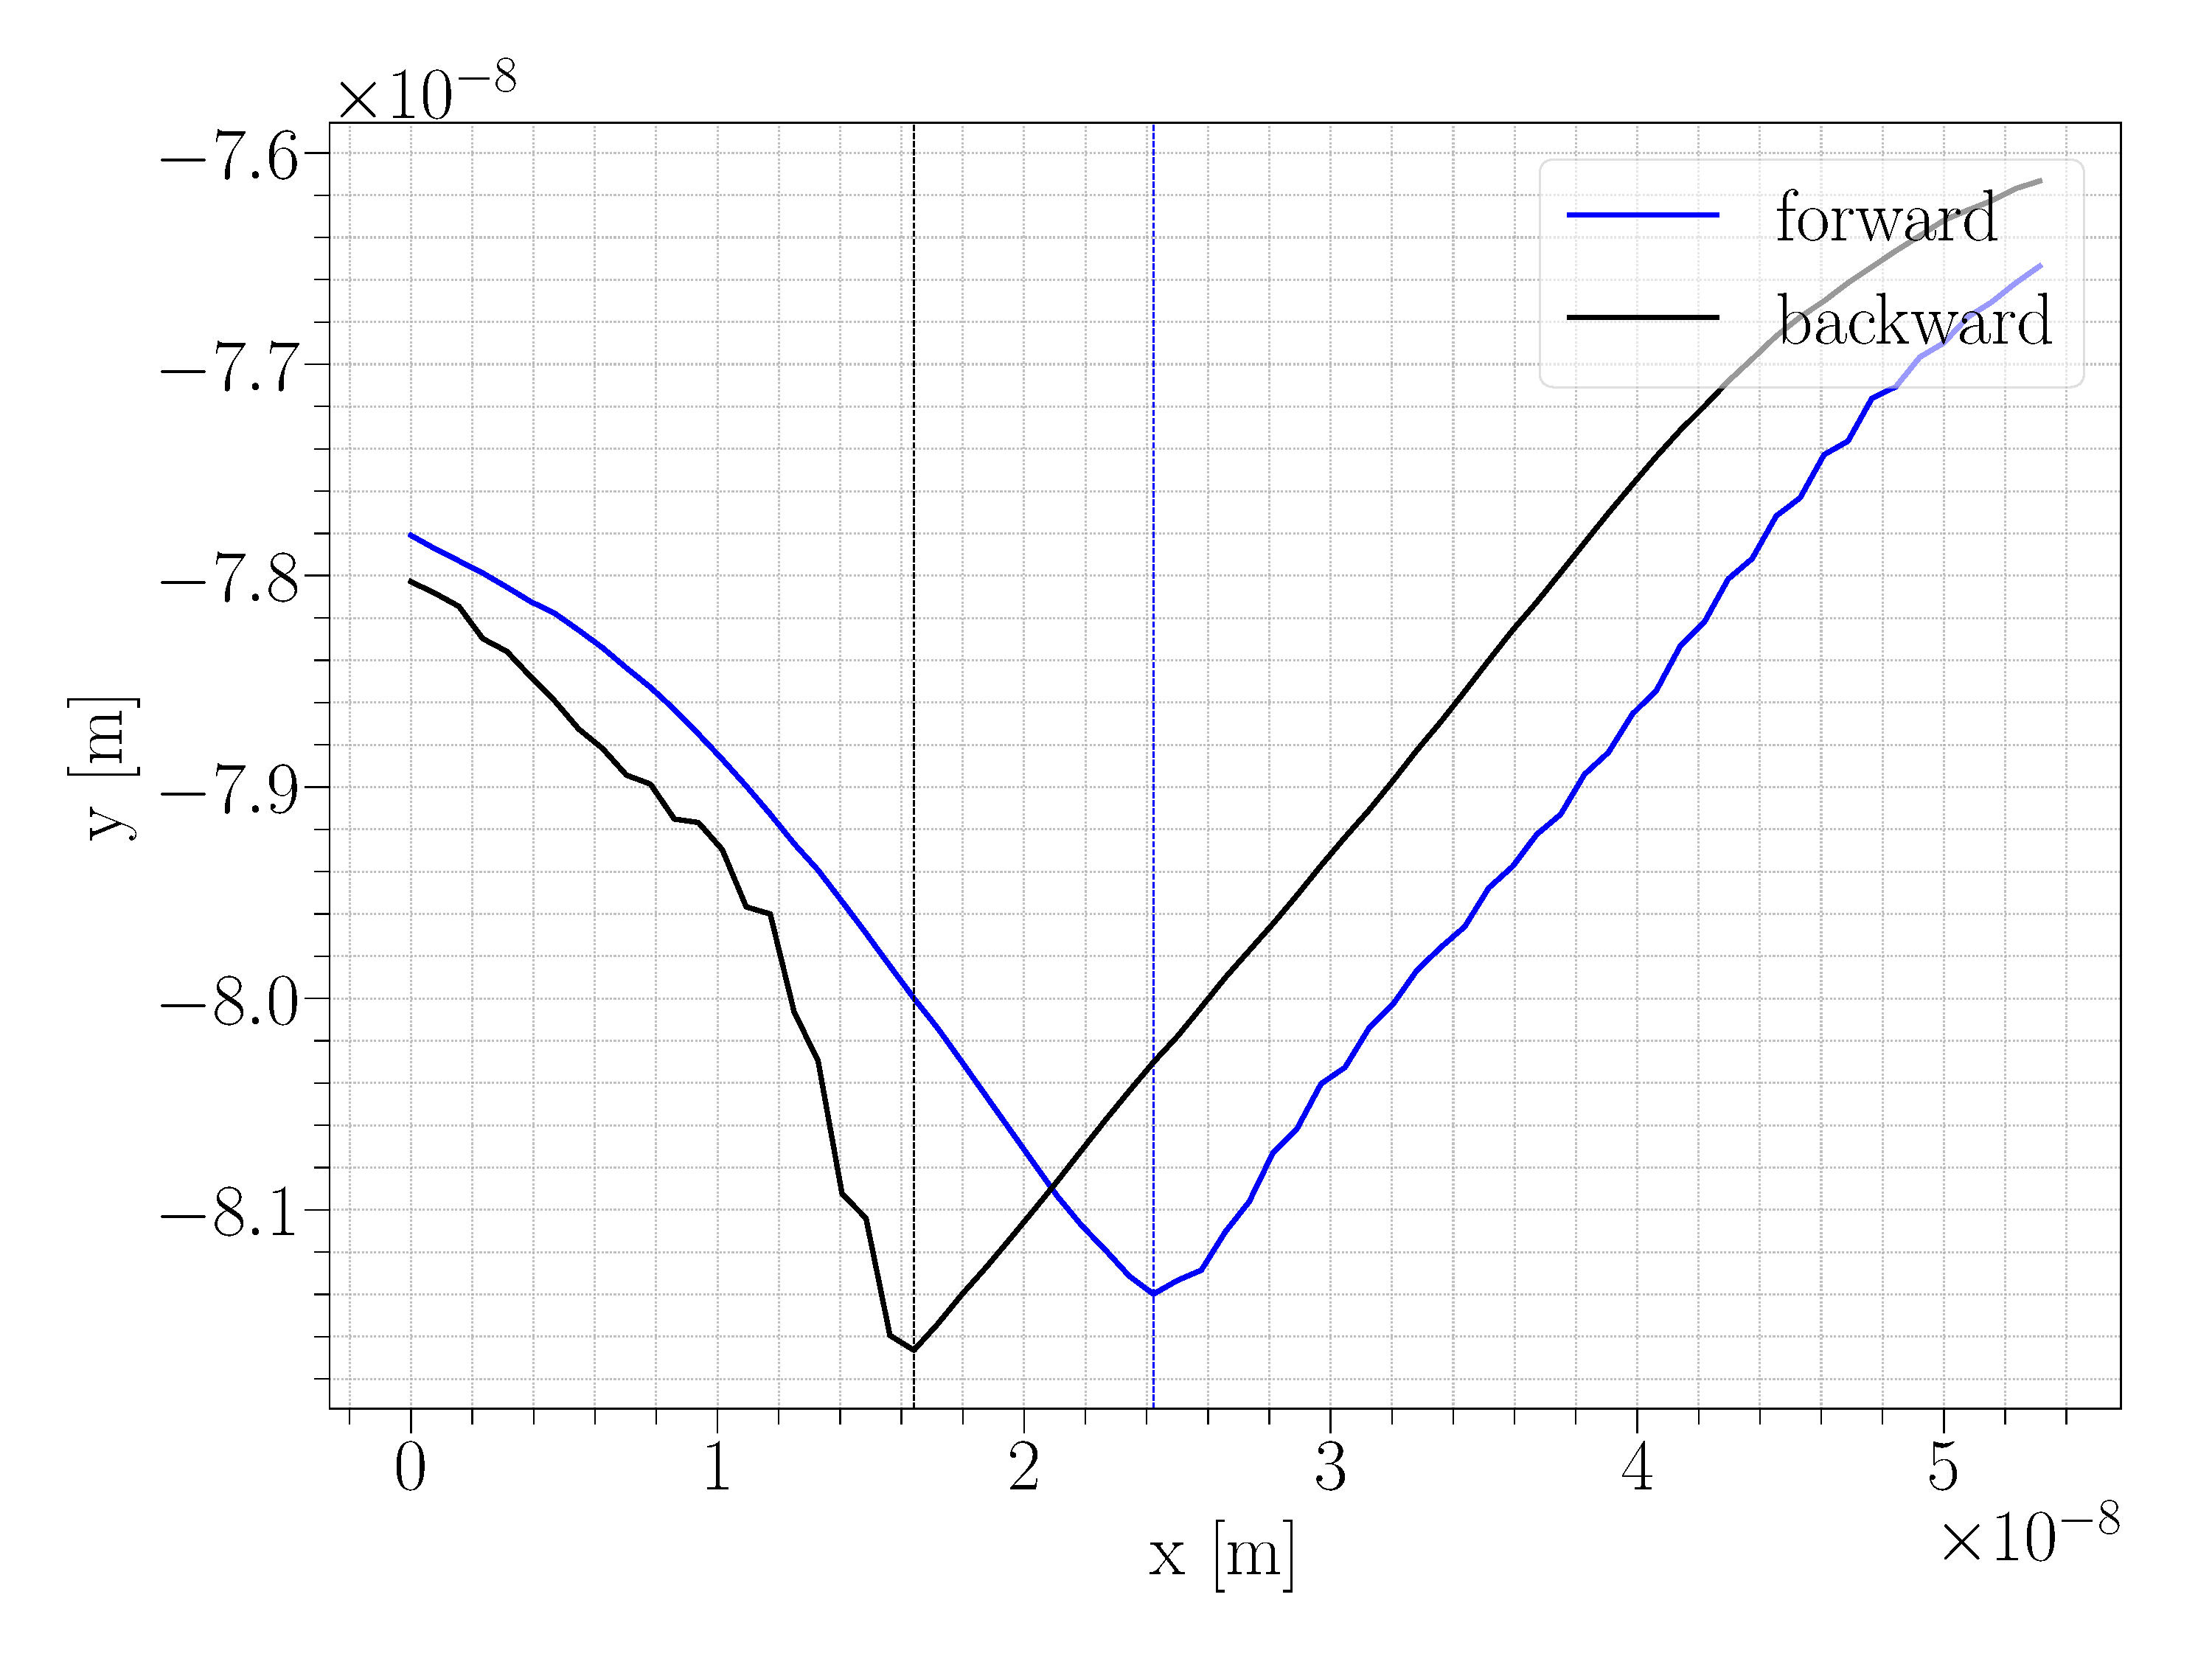
\includegraphics[width=\textwidth]{../Figures/TIME_005_profile.pdf}
\caption{Extrahierte Profile in Vor- und Rückwärtsrichtung für eine Rasterzeit von \SI{0.05}{s}.}
\label{TIME_005_profile}
\end{figure}


TODO: Quantifizierung für zu lange Rasterzeit?


\subsection{Hochorientierter pyrolytischer Graphit (HOPG)}
\subsubsection{Bestimmung der Höhe einer Stufe}

Auf der HOPG Probe wollen wir erstmal eine Stufe finden und ihre Höhe bestimmen. Nachdem wir die z-Bilder mit Gwyddion im Rahmen des Möglichen geebnet hatten, haben wir für jede der drei Auflösungen jeweils drei Profillinien extrahiert, wie exemplarisch in Abbildung \ref{166nm} zu sehen.

Mit Python haben wir aus den Profilen jeweils die mittleren Höhen der Ebenen und ihre Standardabweichung bestimmt (Abbildung \ref{166nmProfiles}). Darauf haben wir die Differenz zwischen hoher und tiefer Ebene berechnet mit quadratisch addierten Standardabweichungen. Abschließend haben wir jeweils aus den drei Höhen das gewichtete Mittel gebildet. Die Ergebnisse sind in Tabelle \ref{tab:heights} zu sehen. Da der Abstand zwischen zwei Schichten in einem Graphitkristall $d = \SI{335}{pm}$ beträgt, würden wir als Höhenunterschied zwischen zwei Ebenen ein Vielfaches davon erwarten. Allerdings spiegeln das unsere Ergebnisse nicht wieder, wie an der starken $\sigma$-Abweichung zu erkennen.

\begin{figure}[H]
\centering
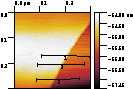
\includegraphics[width=\textwidth]{../Gwyddion/HOPG/300nm.pdf}
\caption{z-Bild bei {300}{nm}-Auflösung. Die Profile wurden entlang der schwarzen Linien extrahiert.}
\label{300nm}
\end{figure}	

\begin{figure}[H]
\centering
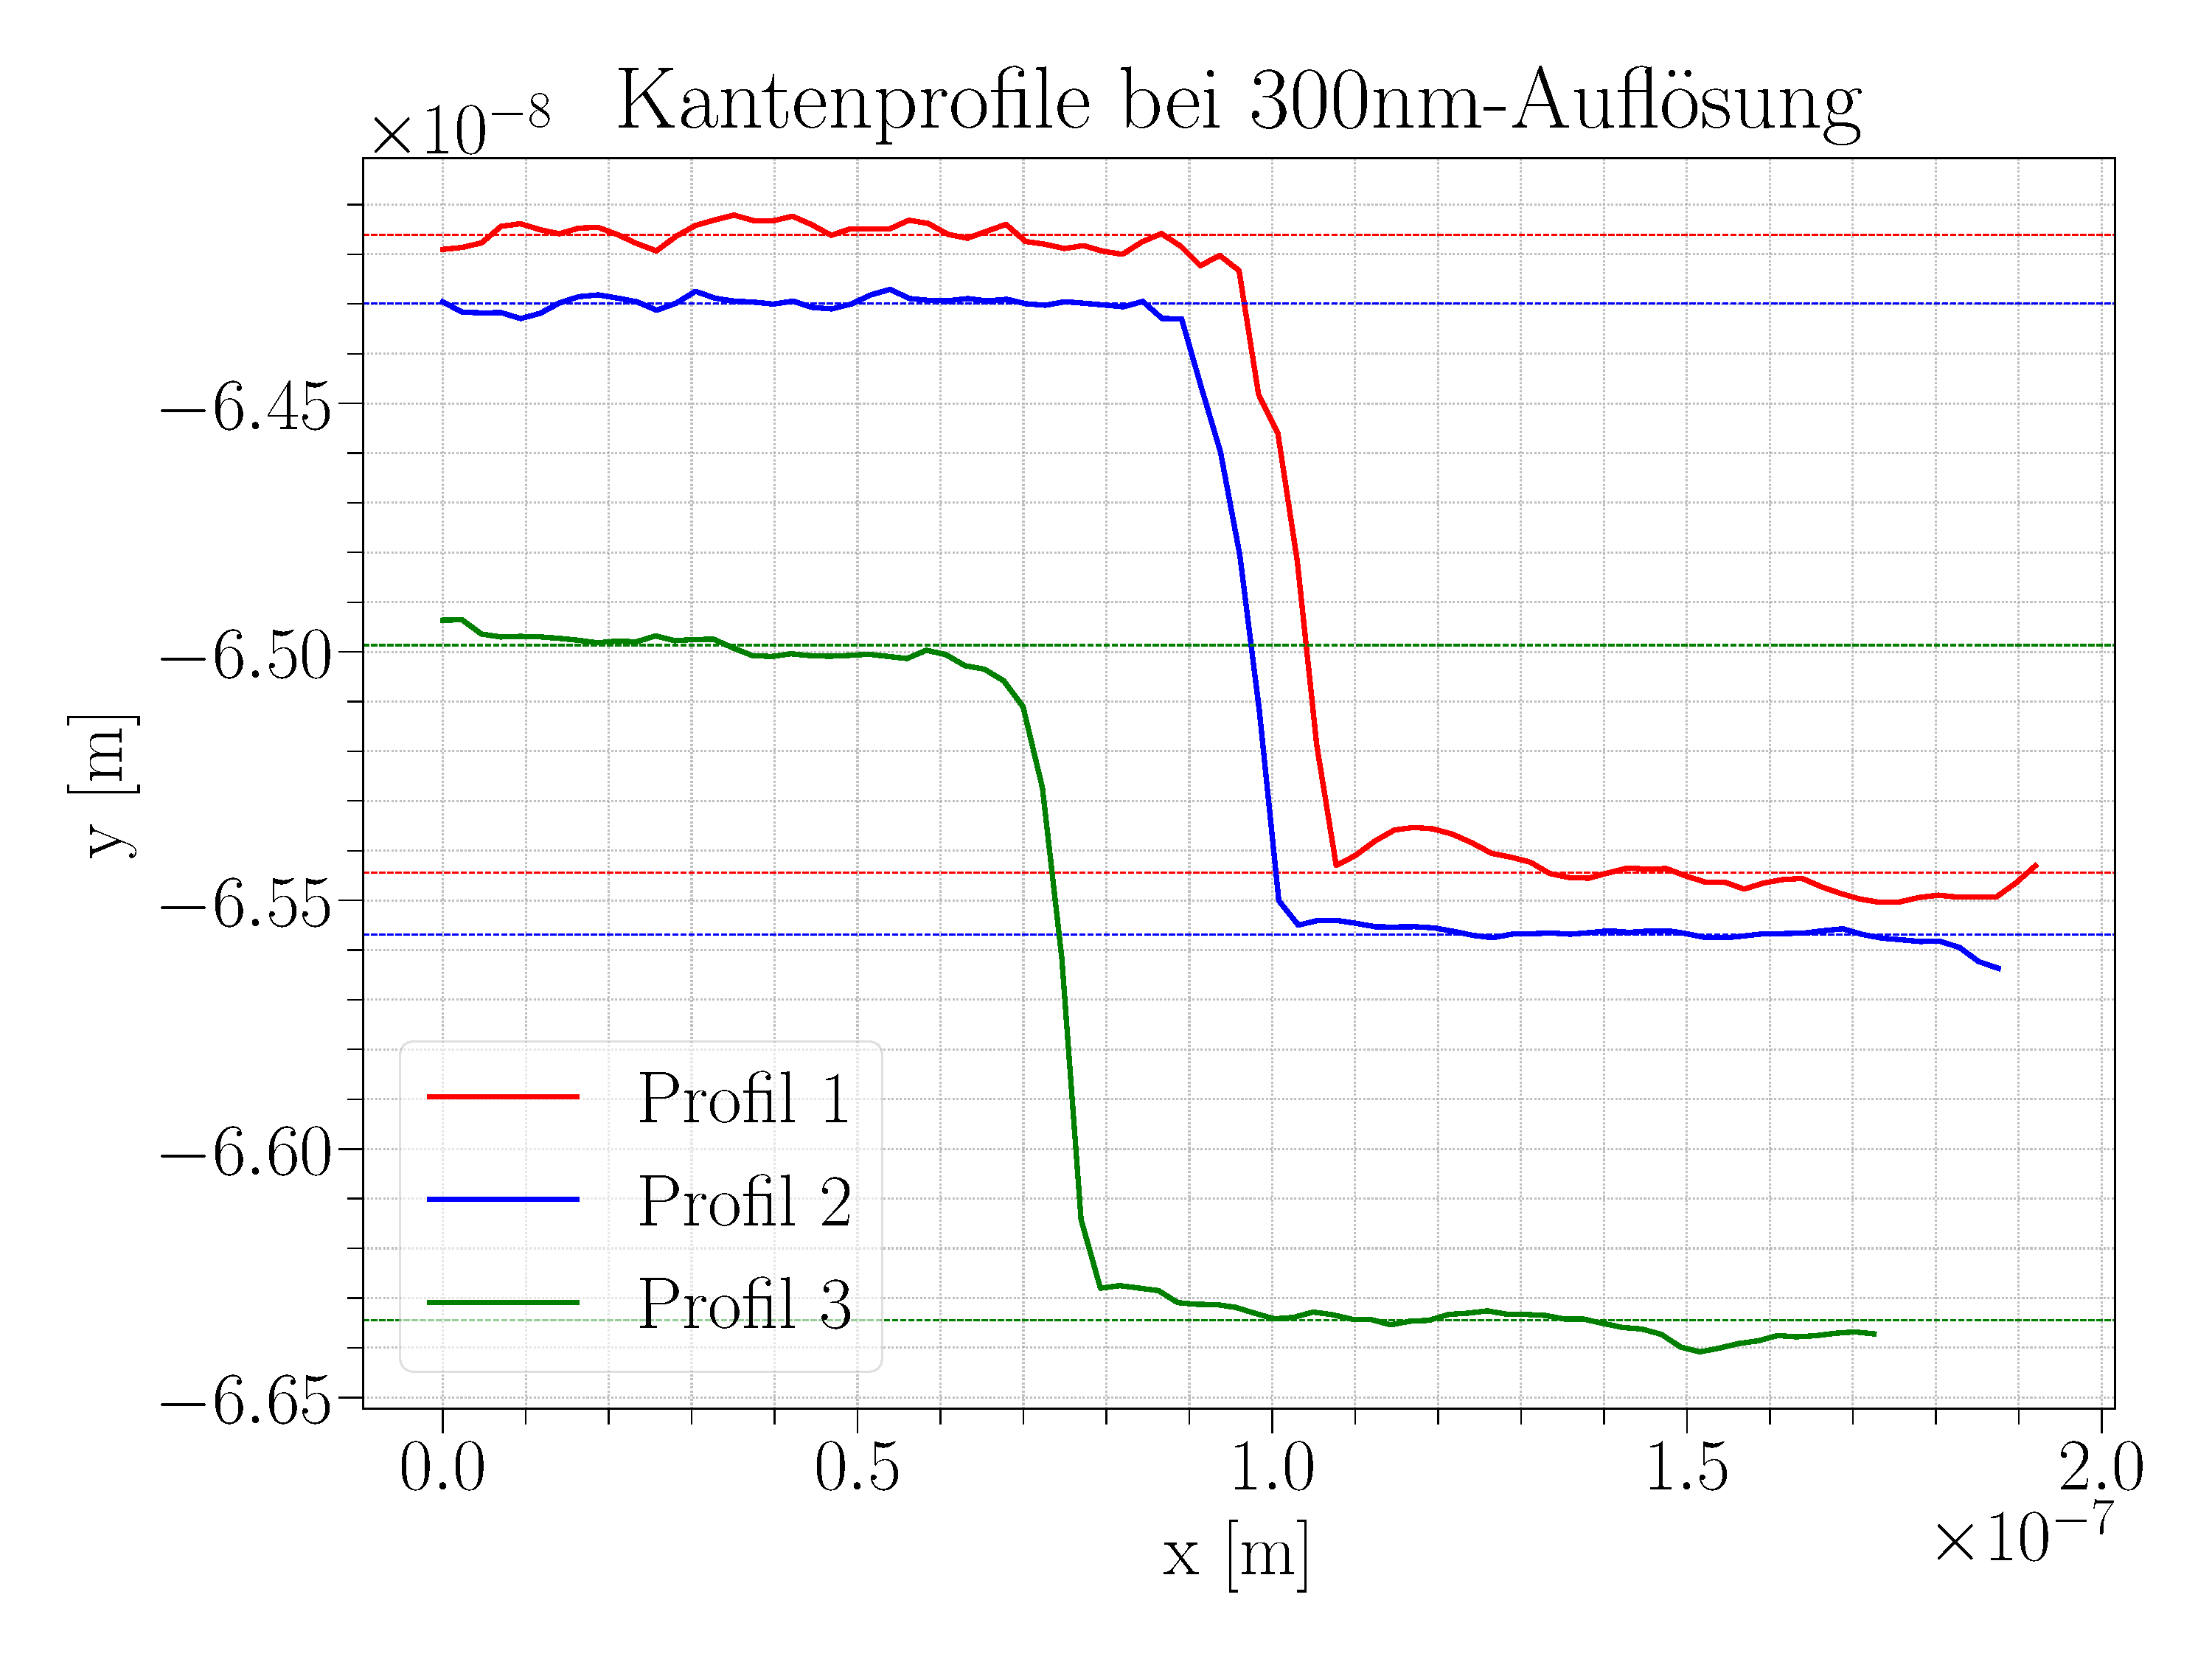
\includegraphics[width=\textwidth]{../Figures/300nm_profiles.pdf}
\caption{Extrahierte Profile bei {300}{nm}-Auflösung.}
\label{300nmProfiles}
\end{figure}	

\begin{figure}[H]
\centering
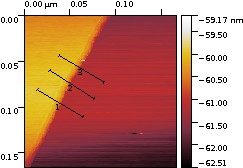
\includegraphics[width=\textwidth]{../Gwyddion/HOPG/166nm.pdf}
\caption{z-Bild bei {166}{nm}-Auflösung. Die Profile wurden entlang der schwarzen Linien extrahiert.}
\label{166nm}
\end{figure}

\begin{figure}[H]
\centering
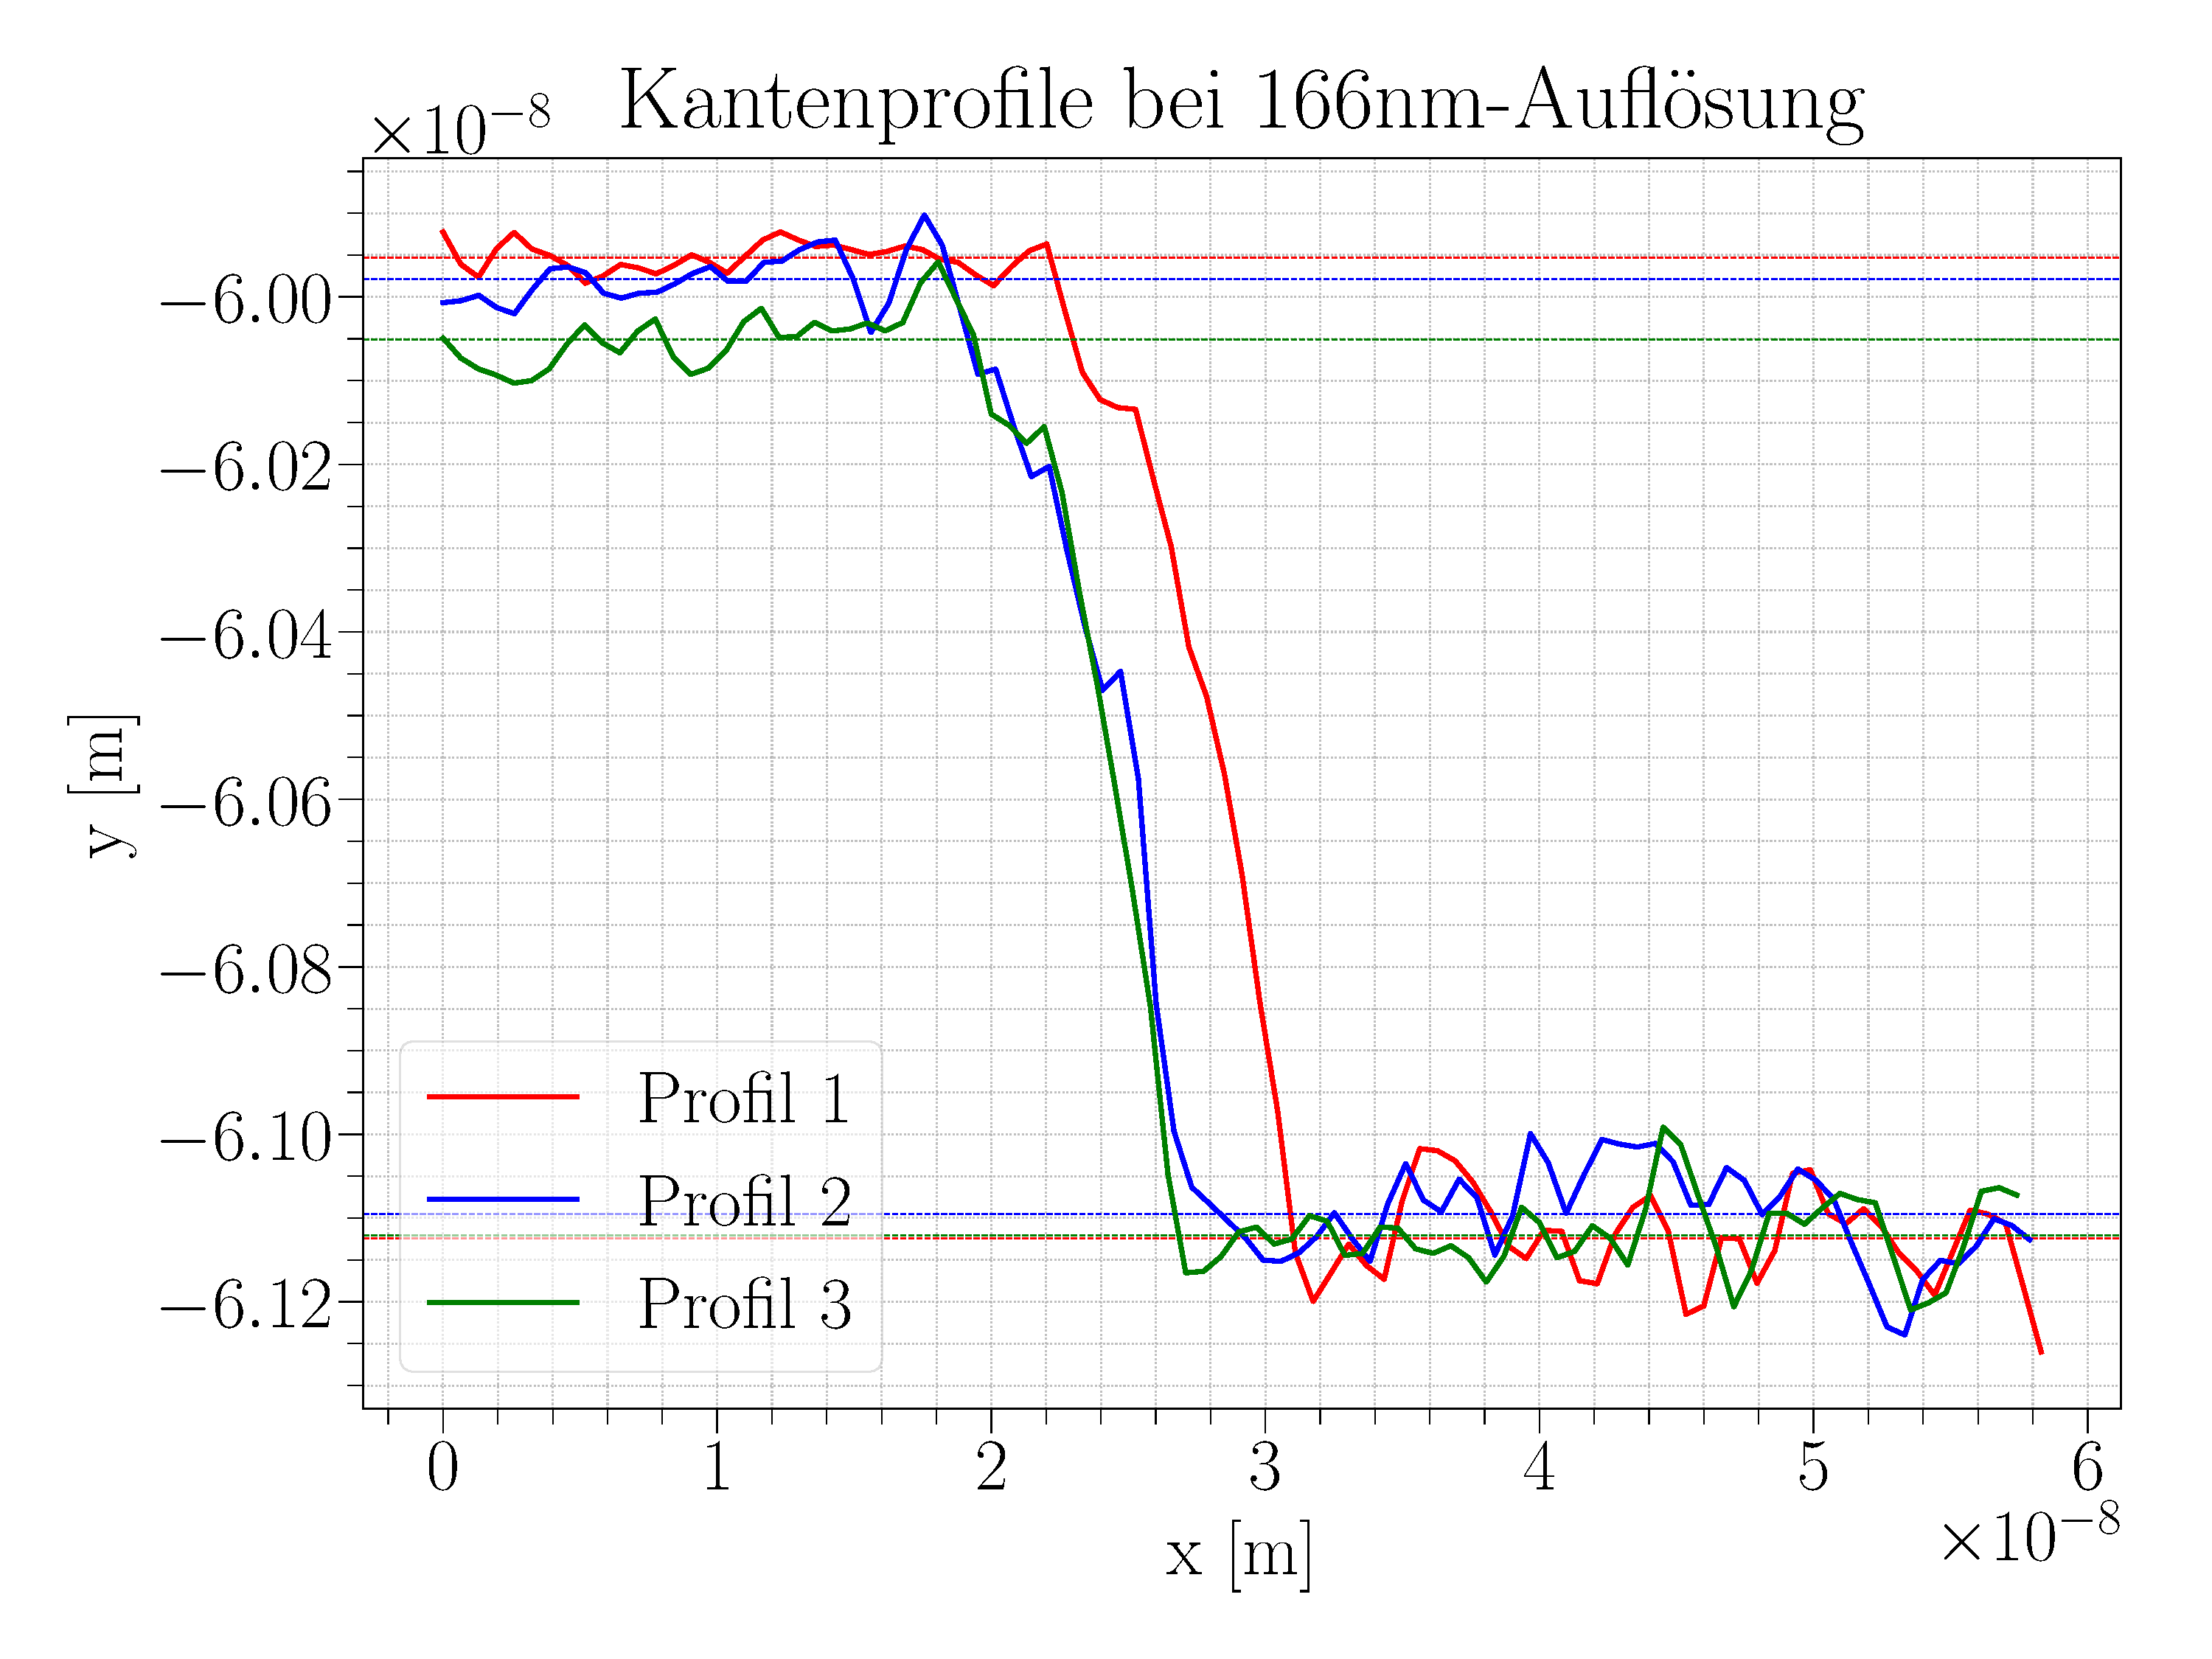
\includegraphics[width=\textwidth]{../Figures/166nm_profiles.pdf}
\caption{Extrahierte Profile bei {166}{nm}-Auflösung.}
\label{166nmProfiles}
\end{figure}

\begin{figure}[H]
\centering
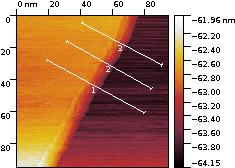
\includegraphics[width=\textwidth]{../Gwyddion/HOPG/95nm.pdf}
\caption{z-Bild bei {95}{nm}-Auflösung. Die Profile wurden entlang der weißen Linien extrahiert.}
\label{95nm}
\end{figure}

\begin{figure}[H]
\centering
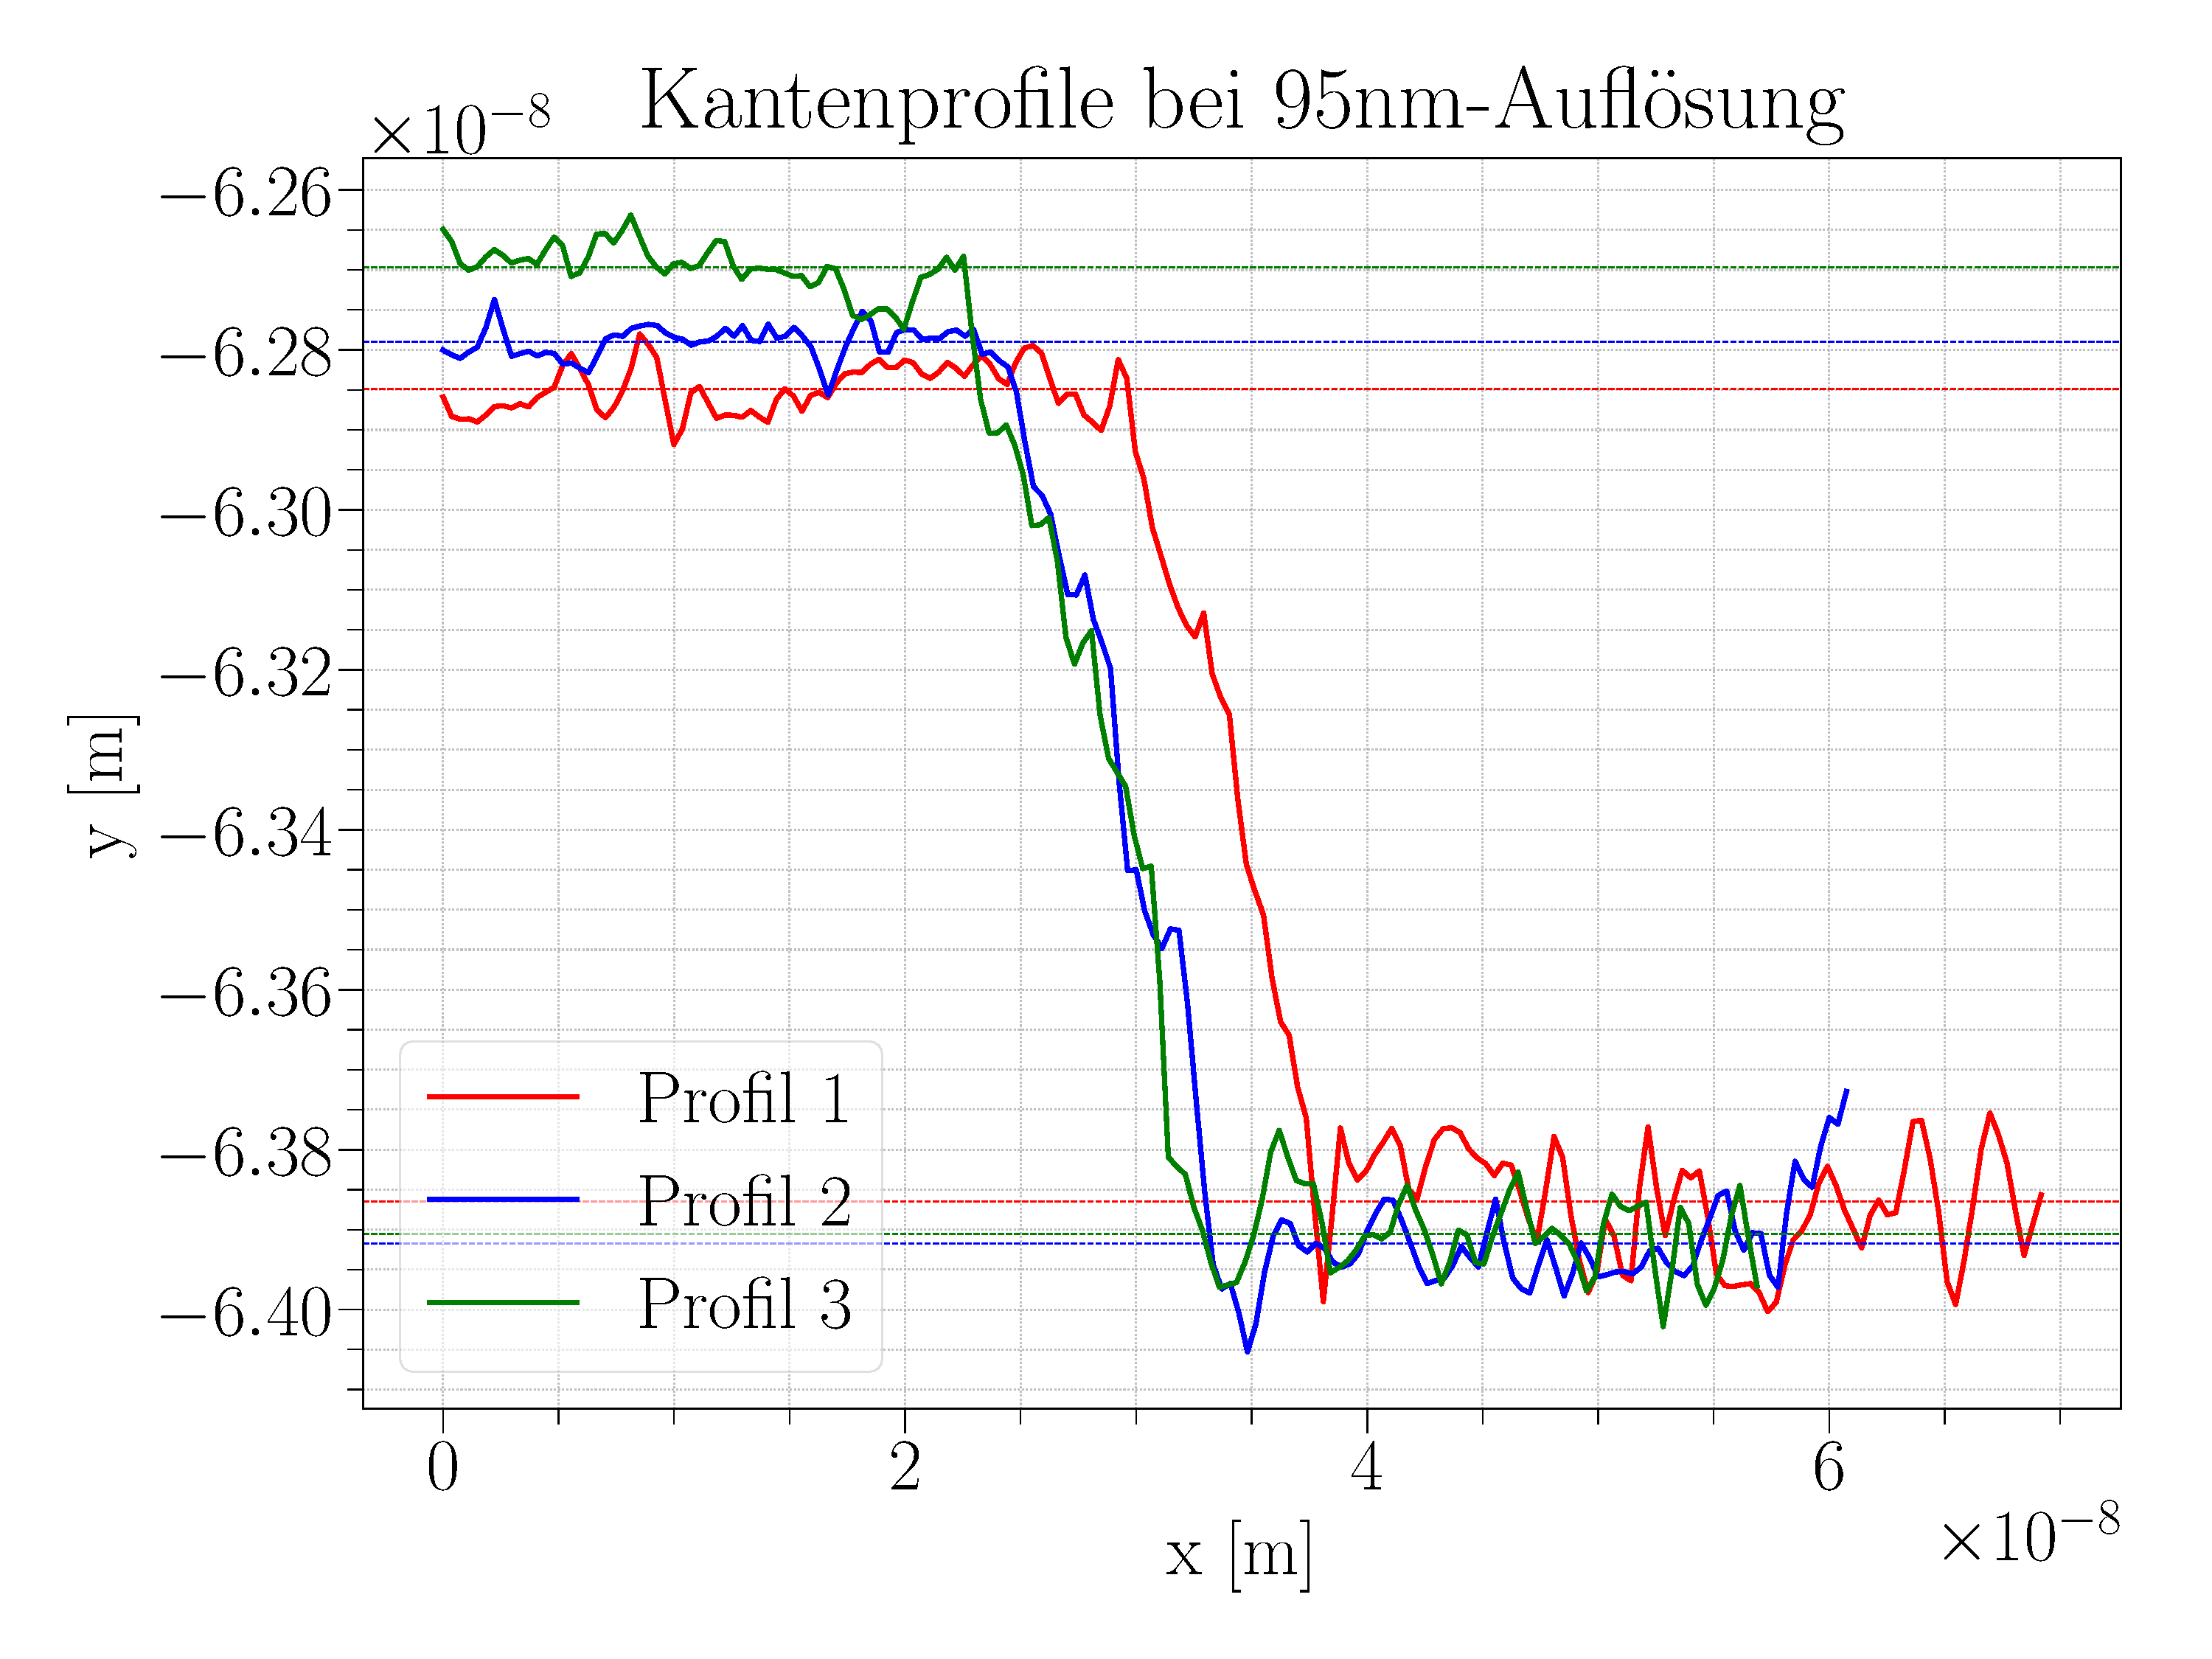
\includegraphics[width=\textwidth]{../Figures/95nm_profiles.pdf}
\caption{Extrahierte Profile bei {95}{nm}-Auflösung.}
\label{95nmProfiles}
\end{figure}

\begin{table}[H]
	\renewcommand{\arraystretch}{1.5}
	\centering
	\begin{tabular}{|c|c|c|c|c|}
		\hline
		Auflösung & individuelle Höhen & gewichtetes Mittel & Abw. von $3d$ & Abw. von $4d$\\
		\hline
		\multirow{3}{*}{\SI{300}{nm}} & \SI{1.283+-0.051}{nm} & \multirow{3}{*}{\SI{1.291+-0.019}{nm}} & \multirow{3}{*}{$\SI{15,1}{\sigma}$} & \multirow{3}{*}{$\SI{2,6}{\sigma}$} \\
		 & \SI{1.270+-0.024}{nm} & & & \\
		 & \SI{1.358+-0.040}{nm} & & & \\
		\hline
		\multirow{3}{*}{\SI{166}{nm}} & \SI{1.172+-0.056}{nm} & \multirow{3}{*}{\SI{1,119+-0,034}{nm}} & \multirow{3}{*}{$\SI{3,4}{\sigma}$} & \multirow{3}{*}{$\SI{6,5}{\sigma}$} \\
		 & \SI{1.117+-0.064}{nm} & & & \\
		 & \SI{1.070+-0.057}{nm} & & & \\
		\hline
		\multirow{3}{*}{\SI{95}{nm}} & \SI{1.016+-0.074}{nm} & \multirow{3}{*}{\SI{1,132+-0,037}{nm}} & \multirow{3}{*}{$\SI{3,4}{\sigma}$} & \multirow{3}{*}{$\SI{5,6}{\sigma}$} \\
		 & \SI{1.127+-0.060}{nm} & & & \\
		 & \SI{1.209+-0.059}{nm} & & & \\
		\hline
	\end{tabular}
	\caption{Ergebnisse für die Stufenhöhe. Wir erwarten ein Vielfaches von $d = \SI{0,335}{nm}$.}
	\label{tab:heights}
\end{table}

\subsubsection{Kalibrierung der x- und y-Achse}

Als Letztes wollen wir mit dem RTM atomar auflösen und dabei die x- und y-Achse kalibrieren. Dafür nutzen wir aus, dass wir die (messbare) Gitterkonstante $g = \SI{246}{pm}$ kennen. Also können wir für jeden gemessenen Abstand $a_{mess}$ zwischen zwei Atomen, zum Beispiel entlang einer zu kalibrirenden Achse, einen erwarteten Abstand $a_{theo}$ angeben.

Seien $a, b, c$ die Kanten eines Dreiecks und $\alpha$ der Winkel zwischen $b$ und $c$, dann lautet der Kosinussatz wie folgt:
\begin{equation}
a^2 = b^2 + c^2 + b \cdot c \cdot \cos\alpha
\end{equation}
Legen wir in den gemessenen Bildern Dreiecke, so dass wir die Atome entlang von $b$ und $c$ abzählen können, erhalten wir
\begin{equation}
a_{theo}^2 = g^2 (N_b^2 + N_c^2 + N_b \cdot N_c \cdot \cos\alpha)
\end{equation}
wobei $N_b, N_c$ die Zahlen der Atome entlang $b, c$ sind, $g$ die Gitterkonstante und in unserem Fall $\alpha = 120^{\circ}$.

Also haben wir für jede Auflösung jeweils drei Dreiecke entlang jeder Achse gelegt, wie in Abbildung \ref{3nm} zu sehen. Außnahme ist die zweite Messung in y-Richtung bei der \SI{2}{nm}-Auflösung. Die Verdrehung der Kristallachse gegenüber der y-Achse ist so gering, dass sich kurze Abstände direkt messen lassen (siehe Abbildung \ref{2nm}). Dann ist $a_{theo} = N \cdot g$.

\begin{figure}[H]
\centering
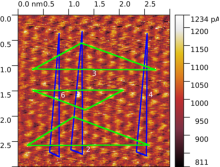
\includegraphics[width=\textwidth]{../Gwyddion/HOPG/3nm_gimped.pdf}
\caption{Strombild bei der \SI{3}{nm}-Auflösung. Dreiecke zur Berechnung von $k_x$ (bzw. $k_y$) sind grün (bzw. blau) eingezeichnet.}
\label{3nm}
\end{figure}

\begin{figure}[H]
\centering
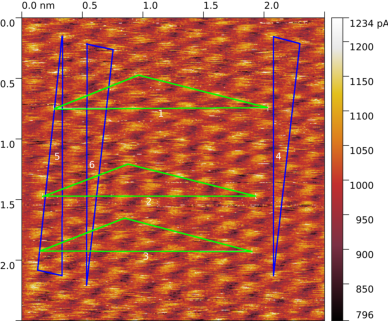
\includegraphics[width=\textwidth]{../Gwyddion/HOPG/2,5nm_gimped.pdf}
\caption{Strombild bei der \SI{2,5}{nm}-Auflösung. Dreiecke zur Berechnung von $k_x$ (bzw. $k_y$) sind grün (bzw. blau) eingezeichnet.}
\label{2,5nm}
\end{figure}

\begin{figure}[H]
\centering
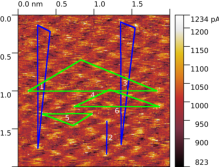
\includegraphics[width=\textwidth]{../Gwyddion/HOPG/2nm_gimped.pdf}
\caption{Strombild bei der \SI{2}{nm}-Auflösung. Dreiecke zur Berechnung von $k_x$ (bzw. $k_y$) sind grün (bzw. blau) eingezeichnet. Die Strecke ohne Dreieck ist mit 2 markiert.}
\label{2nm}
\end{figure}

Da wir das Verhältnis zwischen $a_{mess}$ und $a_{theo}$ als linear annehmen, lässt sich die Kalibrationskonstante direkt aus dem Verhältnis der beiden bestimmen:
\begin{equation}
k = \frac{a_{theo}}{a_{mess}}.
\end{equation}
Wir erhalten so für jedes Dreieck ein $k_{x/y}$. Für jedes Bild bilden wir für $k_x$ und $k_y$ jeweils das gewichtete Mittel. Die einzige Unsicherheit in der Rechnung kommt von der Messung von $a_{mess}$. Da die Position der Mitte der Atome im Bild nicht immer eindeutig ist, haben wir auf die Position in x- bzw. y-Richtung jeweils pro Bild einen Fehler $\sigma_{pos}$ angenommen der etwa einem Atomradius im Bild entspricht. Der Fehler auf $a_{mess}$ ist dann $\sigma_a = \sqrt{2} \cdot \sigma_{pos}$ und pflanzt sich dann gaußisch auf $k$ fort. Die Ergebnisse lassen sich anhand der Tabellen \ref{tab:calibX} und \ref{tab:calibY} nachvollziehen.

\begin{table}[H]
	\renewcommand{\arraystretch}{1.5}
	\centering
	\begin{tabular}{|c|c|c|c|c|}
		\hline
		Auflösung & $a_{mess}$ & $a_{theo}$ & $k_x$ & $\bar{k}_x$ \\
		\hline
		\multirow{3}{*}{\SI{3}{nm}} & \SI{1.78+-0.12}{nm} & \SI{1.27}{nm} & \SI{0.71+-0.05}{nm} & \multirow{3}{*}{\SI{0.72+-0.03}{nm}} \\
		 & \SI{2.41+-0.12}{nm} & \SI{1.76}{nm} & \SI{0.73+-0.04}{nm} & \\
		 & \SI{2.43+-0.12}{nm} & \SI{1.76}{nm} & \SI{1.72+-0.04}{nm} & \\
		\hline
		\multirow{3}{*}{\SI{2,5}{nm}} & \SI{1.77+-0.13}{nm} & \SI{1.27}{nm} & \SI{0.71+-0.06}{nm} & \multirow{3}{*}{\SI{0.72+-0.03}{nm}} \\
		 & \SI{1.76+-0.13}{nm} & \SI{1.27}{nm} & \SI{0.72+-0.06}{nm} & \\
		 & \SI{1.75+-0.13}{nm} & \SI{1.27}{nm} & \SI{0.72+-0.06}{nm} & \\
		\hline
		\multirow{3}{*}{\SI{2}{nm}} & \SI{1.71+-0.12}{nm} & \SI{1.27}{nm} & \SI{0.74+-0.05}{nm} & \multirow{3}{*}{\SI{0.73+-0.04}{nm}} \\
		 & \SI{0.66+-0.12}{nm} & \SI{0.49}{nm} & \SI{0.75+-0.13}{nm} & \\
		 & \SI{1.12+-0.12}{nm} & \SI{0.78}{nm} & \SI{0.69+-0.07}{nm} & \\
		\hline
	\end{tabular}
	\caption{Ergebnisse für die Kalibrierung der x-Achse.}
	\label{tab:calibX}
\end{table}

\begin{table}[H]
	\renewcommand{\arraystretch}{1.5}
	\centering
	\begin{tabular}{|c|c|c|c|c|}
		\hline
		Auflösung & $a_{mess}$ & $a_{theo}$ & $k_y$ & $\bar{k}_y$ \\
		\hline
		\multirow{3}{*}{\SI{3}{nm}} & \SI{2.42+-0.09}{nm} & \SI{2.67}{nm} & \SI{1.10+-0.04}{nm} & \multirow{3}{*}{\SI{1.09+-0.03}{nm}} \\
		 & \SI{2.43+-0.09}{nm} & \SI{2.67}{nm} & \SI{1.09+-0.04}{nm} & \\
		 & \SI{2.45+-0.09}{nm} & \SI{2.67}{nm} & \SI{1.08+-0.04}{nm} & \\
		\hline
		\multirow{3}{*}{\SI{2,5}{nm}} & \SI{1.98+-0.09}{nm} & \SI{3.15}{nm} & \SI{1.59+-0.07}{nm} & \multirow{3}{*}{\SI{1.59+-0.04}{nm}} \\
		 & \SI{1.97+-0.09}{nm} & \SI{3.15}{nm} & \SI{1.59+-0.07}{nm} & \\
		 & \SI{1.99+-0.09}{nm} & \SI{3.15}{nm} & \SI{1.58+-0.07}{nm} & \\
		\hline
		\multirow{3}{*}{\SI{2}{nm}} & \SI{1.62+-0.08}{nm} & \SI{1.68}{nm} & \SI{1.03+-0.05}{nm} & \multirow{3}{*}{\SI{1.04+-0.04}{nm}} \\
		 & \SI{0.43+-0.08}{nm} & \SI{0.49}{nm} & \SI{1.14+-0.19}{nm} & \\
		 & \SI{1.62+-0.08}{nm} & \SI{1.68}{nm} & \SI{1.03+-0.05}{nm} & \\
		\hline
	\end{tabular}
	\caption{Ergebnisse für die Kalibrierung der y-Achse.}
	\label{tab:calibY}
\end{table}

Alle $\bar{k}_x$ sind miteinander innerhalb einer 1$\sigma$-Abweichung kompatibel. Bei den $\bar{k}_y$ sind die Werte für die \SI{3}{nm}- und \SI{2}{nm}-Auflösung innerhalb einer 1$\sigma$-Abweichung kompatibel aber der Wert für die \SI{2,5}{nm}-Auflösung weicht sehr stark von den anderen ab. Die Abweichung fällt schon bei der Betrachtung der gemessenen Abstände auf. Diese müssten, nach Betrachtung der $a_{theo}$, im Vergleich zu den Messungen bei \SI{3}{nm} größer sein. Entweder die Messung war fehlerhaft oder die y-Achse verhält sich nicht linear. In beiden Fällen würden sich erneute Messungen lohnen.


\section{Fazit}

Der Versuch war insofern erfolgreich, dass die Experimentatoren sich mit der Funktionsweise des RTM und mit entsprechender Auswertungssoftware vertraut gemacht haben.

Wenn wir uns die konkreten Ergebnisse anschauen, ist das Fazit durchwachsener. Die gefundenen Stufenhöhen bei HOPG widersprechen der Erwartung. Da nur zwei von drei Stufenhöhen bei verschiedenen Auflösungen miteinander konsistent sind, wäre eine erneute Messung angebracht.

Die Ergebnisse für die Kalibrierungskonstanten sind, bis auf $k_y$ für die \SI{2}{nm}-Auflösung, miteinander verträglich und könnten als solche verwendet werden. Lediglich das abweichende $k_y$ sollte lieber in einer neuen Messung bestimmt werden. Wenn das Ergebnis dennoch bestätigt würde, hätten wir es mit einem nicht-linearen Verhalten der y-Achse zu tun.

\end{document}
